\documentclass[conference]{IEEEtran}
\IEEEoverridecommandlockouts
% The preceding line is only needed to identify funding in the first footnote. If that is unneeded, please comment it out.
\usepackage{cite}
\ifCLASSOPTIONcompsoc \usepackage[caption=false,font=normalsize,labelfon
t=sf,textfont=sf]{subfig}
\else
\usepackage[caption=false,font=footnotesize]{subfi g}
\fi
\usepackage{amsmath,amssymb,amsfonts}
\usepackage{algorithmic}
\usepackage{graphicx}
\usepackage{textcomp}
\usepackage{xcolor}
\def\BibTeX{{\rm B\kern-.05em{\sc i\kern-.025em b}\kern-.08em
    T\kern-.1667em\lower.7ex\hbox{E}\kern-.125emX}}
\begin{document}

\title{Control of a Three Degree of Freedom Quadcopter Stand Using Linear Quadratic Integral Based on the Differential Game Theory\\
% {\footnotesize \textsuperscript{*}Note: Sub-titles are not captured in Xplore and
% should not be used}
\thanks{In partnership with BaniAsad Industries}
}

\author{\IEEEauthorblockN{Hadi Nobahari}
\IEEEauthorblockA{\textit{Department of Aerospace Engineering} \\
\textit{Sharif University of Technology}\\
Tehran, Iran \\
nobahari@sharif.edu}
\and
\IEEEauthorblockN{Ali BaniAsad}
\IEEEauthorblockA{\textit{Department of Aerospace Engineering} \\
\textit{Sharif University of Technology}\\
Tehran, Iran \\
alibaniasad1999@yahoo.com}
% \and
% \IEEEauthorblockN{3\textsuperscript{rd} Given Name Surname}
% \IEEEauthorblockA{\textit{dept. name of organization (of Aff.)} \\
% \textit{name of organization (of Aff.)}\\
% City, Country \\
% email address or ORCID}
% \and
% \IEEEauthorblockN{4\textsuperscript{th} Given Name Surname}
% \IEEEauthorblockA{\textit{dept. name of organization (of Aff.)} \\
% \textit{name of organization (of Aff.)}\\
% City, Country \\
% email address or ORCID}
% \and
% \IEEEauthorblockN{5\textsuperscript{th} Given Name Surname}
% \IEEEauthorblockA{\textit{dept. name of organization (of Aff.)} \\
% \textit{name of organization (of Aff.)}\\
% City, Country \\
% email address or ORCID}
% \and
% \IEEEauthorblockN{6\textsuperscript{th} Given Name Surname}
% \IEEEauthorblockA{\textit{dept. name of organization (of Aff.)} \\
% \textit{name of organization (of Aff.)}\\
% City, Country \\
% email address or ORCID}
}

\maketitle

\begin{abstract}
    In this paper, a quadcopter stand with three degrees of freedom was controlled using game theory-based control. The first player tracks a desired input, and the second player creates a disturbance in the tracking of the first player to cause an error in the tracking. The ???? move is chosen using the Nash equilibrium, which presupposes that the other player made the worst move. In addition to being resistant to input interruptions, this method may also be resilient to modeling system uncertainty. This method evaluated the performance through simulation in the Simulink environment and implementation on a three-degree-of-freedom stand.
\end{abstract}

\begin{IEEEkeywords}
    Quadcopter, Differential Game, Game Theory, Nash Equilibrium, Three Degree of Freedom Stand, Model Base Design, Linear Quadratic Regulator
\end{IEEEkeywords}

\section{Introduction}
% This document is a model and instructions for \LaTeX.
% Please observe the conference page limits. 
Quadcopter is a type of helicopter with four rotors. % https://en.wikipedia.org/wiki/Quadcopter#cite_note-dasc04-1


\section{Differential Game}
Differential games are a series of problems that arise while examining and simulating dynamic systems in game theory.
%  A differential game is a game in which the player who is trying to maximize the utility of his strategy is the opponent. The player who is trying to minimize the utility of his strategy is the player who is trying to maximize the utility of the opponent's strategy.
% In the context of differential games, differential games in game theory address the modeling and analysis of dynamic systems.
% Differential games are a class of games in which the players are able to model the system and the players are able to choose the optimal move.
% Differential games are sets of issues that arise while examining and simulating dynamic systems in game theory.
Differential equations
%  are used to 
 simulate how a state variable or set of state variables changes over time.
% Differential equations are used to model the evolution over time of a state variable or variables.
\subsection{An introduction to the differential game}
It is considered that two players are involved in this research.
% In this paper, there are considered to be two players.
The space states of a continuous linear system are shown below.
\begin{equation}\label{system_dynamic}
    \begin{split}
             &\boldsymbol{\dot{\mathrm{x}}}(t) = \boldsymbol{\mathrm{Ax}}(t) + \boldsymbol{\mathrm{B_1u_1}}(t) + \boldsymbol{\mathrm{B_2u_2}}(t)%, \quad \boldsymbol{x}(0) = \boldsymbol{x}_0
        \\
        &\boldsymbol{\mathrm{y}}(t) = \boldsymbol{\mathrm{Cx}}(t) + \boldsymbol{\mathrm{D_1u_1}}(t) + \boldsymbol{\mathrm{D_2u_2}}(t)
    \end{split}
\end{equation}
Where $\boldsymbol{\mathrm{x}}$ is the vector of the state variables, $\boldsymbol{\dot{\mathrm{x}}}$ is the time derivative of the state vector, $\boldsymbol{\mathrm{u_1}}$ is the first player (controller) input vector, $\boldsymbol{\mathrm{u_2}}$ is the second player (disturbance) input vector, $\boldsymbol{\mathrm{y}}$ is the output vector, $\boldsymbol{\mathrm{A}}$ is the state matrix, $\boldsymbol{\mathrm{B_1}}$ is the first player input matrix, $\boldsymbol{\mathrm{B_2}}$ is the second player input matrix,
$\boldsymbol{\mathrm{C}}$ is the output matrix, $\boldsymbol{\mathrm{D_1}}$ is first player the output matrix and $\boldsymbol{\mathrm{D_2}}$ is second player the output matrix.
Equation \eqref{system_dynamic} demonstrates how both participants have an impact on the system's dynamics.
% As shown in equation 1, both players affect the dynamics of the system.
The second player may progress toward the goal as a result of the first player's exertion, or vice versa.
% The first player's effort could push the second player away from the goal, or the other way around.
This paper considers the case that players do not cooperate in order to realize their goals.
The situation where players do not work together (non-cooperative) to achieve their objectives is examined in the paper.
% The paper examines the situation in which players do not cooperate to achieve their goals.
In this case, every player knows at time $t \in [0, T]$ just the initial state $\boldsymbol{\mathrm{x}_0}$ and the model structure.
% This scenario can be interpreted as the players simultaneously determining their actions, next submitting their actions. 
% The players can be interpreted as simultaneously determining their actions, then submitting them.
For the game (1,2), we will use the set of Nash equilibria. Formal Nash equilibrium is defined as follows.
% Here are the formal Nash equilibrium definitions for games (1) and (2).
% defenition
An admissible set of actions $(\boldsymbol{u_1}^*,  \boldsymbol{u_2}^*)$ is a Nash equilibrium for the game (1,2); if for all admissible $(\boldsymbol{u_1},  \boldsymbol{u_2})$, the following inequalities hold:
\begin{equation}\label{nash_lqe}
	J_1(\boldsymbol{\mathrm{u_1}}^*, \boldsymbol{\mathrm{u_2}}^*)\leq J_1(\boldsymbol{\mathrm{u_1}}, \boldsymbol{\mathrm{u_2}}^*) \text{\rm{ , }}
	J_2(\boldsymbol{\mathrm{u_1}}^*, \boldsymbol{\mathrm{u_2}}^*)\leq 
	J_2(\boldsymbol{\mathrm{u_1}}^*, \boldsymbol{\mathrm{u_2}})
\end{equation}
% Here admissibility is meant in the sense that $\boldsymbol{\mathrm{u_i}}(.)$ belongs to some restricted set, where this set depends on the information players have on the game, the set of strategies the players like to use to control the system, and the system (2) must have a unique solution.
% The term admissibility refers to the fact that u(.) belongs to a restricted set determined by the information players have about the game, the strategies they use to control the system, and the uniqueness of the solution.
\subsection{LQDG controller}
For the system described in equation \eqref{system_dynamic}, LQDG optimum control effort calculates from equation \eqref{LQDG_u}.
% The optimum control effort calculated by LQDG for the system described in equation 1 is calculated using equation 2.
% For the system described in equation 1, LQDG optimum control effort calculates from equation 2.
\begin{equation}\label{LQDG_u}
	\boldsymbol{\mathrm{u_i}}(t) = -\boldsymbol{\mathrm{R_{ii}}}^{-1}\boldsymbol{\mathrm{B_i}}^\mathrm{T}\boldsymbol{\mathrm{P_{i}}}(t)\boldsymbol{\mathrm{x}}(t) = -\boldsymbol{\mathrm{K_{i}}}(t)\boldsymbol{\mathrm{x}}(t),\quad i = 1, 2
\end{equation}
In equation \eqref{LQDG_u}, $\boldsymbol{\mathrm{K_{i}}}$ is the optimal feedback gain. Assuming that the other players will make their worst move, this gain is calculated to minimize the quadratic cost function equation \eqref{cost} of player number i.
\begin{equation}\label{cost}
    \begin{split}
        J_i( \boldsymbol{\mathrm{u_1}},  \boldsymbol{\mathrm{u_2}}) = \int_{0}^{T}\biggl (\boldsymbol{\mathrm{x}} ^\mathrm{T}(t) \boldsymbol{\mathrm{Q_i}} \boldsymbol{\mathrm{x}}(t)+
        &\boldsymbol{\mathrm{u_i}} ^\mathrm{T}(t) \boldsymbol{\mathrm{R_{ii}}} \boldsymbol{\mathrm{u_i}}(t)+\\
        &\boldsymbol{\mathrm{u_j}} ^\mathrm{T}(t)\boldsymbol{\mathrm{ R_{ij} u_j}}(t)
        \biggl )\mathrm{d}t
    \end{split} 
\end{equation}
Here the matrices $\boldsymbol{\mathrm{Q_i}}$ and  $\boldsymbol{\mathrm{R_{ii}}}$ are assumed to be symmetric and $\boldsymbol{\mathrm{R_{ii}}}$ positive definite.
$\boldsymbol{\mathrm{P_{i}}}$ is found by solving the continuous time couple Riccati differential equation:
\begin{equation}\label{coupled_riccatti_LQDG}
	\begin{split}
		&\begin{split}
             \boldsymbol{\dot{\mathrm{P}}_1}(t) = -&\boldsymbol{\mathrm{A}}^\mathrm{T}\boldsymbol{\mathrm{P_1}}(t) - \boldsymbol{\mathrm{P_1}}(t)\boldsymbol{\mathrm{A}} - \boldsymbol{\mathrm{Q_1}} +\boldsymbol{\mathrm{P_1}}(t)\boldsymbol{\mathrm{S_1}}(t)\boldsymbol{\mathrm{P_1}}(t) +\\ &\boldsymbol{\mathrm{P_1}}(t)\boldsymbol{\mathrm{S_2}}(t)\boldsymbol{\mathrm{P_2}}(t)
		\end{split}\\
		&\begin{split}
            \boldsymbol{\dot{\mathrm{P}}_2}(t) = -&\boldsymbol{\mathrm{A}}^\mathrm{T}\boldsymbol{\mathrm{P_2}}(t) - \boldsymbol{\mathrm{P_2}}(t)\boldsymbol{\mathrm{A}} - \boldsymbol{\mathrm{Q_2}} +\boldsymbol{\mathrm{P_2}}(t)\boldsymbol{\mathrm{S_2}}(t)\boldsymbol{\mathrm{P_2}}(t) +\\ &\boldsymbol{\mathrm{P_2}}(t)\boldsymbol{\mathrm{S_1}}(t)\boldsymbol{\mathrm{P_1}}(t)
		\end{split}
	\end{split}
\end{equation}
Using the shorthand notation $\boldsymbol{S_i} := \boldsymbol{B_iR_{ii}}^{-1}\boldsymbol{B_i}^\mathrm{T}$. %?????????????????????


\subsection{LQIDG controller}
The absence of an integrator in the LQDG controller may result in steady-state errors due to disturbances or modeling errors.
% The LQDG controller's lack of an integrator could lead to steady-state errors due to disturbances or faulty modeling.
The LQIDG controller is based on the LQDG controller to eliminate this error.

The LQIDG controller adds the integral of the difference between the system output and the desired value to the state vector.
% In this controller, the integral of the difference between the system output and the desired value is added to the state vector.
% The integral of the difference between the system output and the desired value is added to the state vector by the LQIDG controller.
Therefore, The augmented space states of a continuous linear system are shown below.
\begin{equation}\label{lqidg_x}
    \boldsymbol{\mathrm{x_a}} = \begin{bmatrix}
        \boldsymbol{\mathrm{x_d}} - \boldsymbol{\mathrm{x}}\\
        \displaystyle \int (\boldsymbol{\mathrm{y_d}} - \boldsymbol{\mathrm{y}})
    \end{bmatrix}
\end{equation}
Where $\boldsymbol{\mathrm{x_a}}$ is the vector of augmented state variables, $\boldsymbol{\mathrm{x_d}}$ is the vector of the desired state variables, and $\boldsymbol{\mathrm{y_d}}$ is the desired output vector.
As a result, the state vector and the output vector are equal.
% Hence, the output vector equals the state vector.
\begin{equation}
	\boldsymbol{\mathrm{y}} = \boldsymbol{\mathrm{x}}
\end{equation}
The following represents the system dynamics in the augmented state space.
% Following is a representation of the system dynamics in the augmented state space.
% In the augmented state space, the system's dynamics are shown below.
\begin{equation}\label{systemlqidg}
	\begin{split}
		\boldsymbol{\dot{\mathrm{x}}_a}(t) &= \boldsymbol{\mathrm{A_ax_a}}(t) + \boldsymbol{\mathrm{B_{{a_1}}u_{a_1}}}(t) + \boldsymbol{\mathrm{B_{{a_2}}u_{a_2}}}(t)%, \quad \boldsymbol{x}(0) = \boldsymbol{x}_0%
		% \\
		% \boldsymbol{\mathrm{y}}(t) &= \boldsymbol{\mathrm{C_ax_a}}(t) + \boldsymbol{\mathrm{D_{{a_1}}u_{a_1}}}(t) + \boldsymbol{\mathrm{D_{{a_2}}u_{a_2}}}(t)
	\end{split}
\end{equation}
Where matrices $\boldsymbol{\mathrm{A_a}}$ and $\boldsymbol{\mathrm{B_a}}$ are defined as follows:
\begin{equation}
	\boldsymbol{\mathrm{A_a}} = \begin{bmatrix}
		\boldsymbol{\mathrm{A}} &0\\
		\boldsymbol{\mathrm{C}} & 0
	\end{bmatrix}
, \quad
	\boldsymbol{\mathrm{B_a}} = \begin{bmatrix}
		\boldsymbol{\mathrm{B}}\\
		0
	\end{bmatrix}
\end{equation}
By introducing a new space state for the system, the remaining design phases of the LQIDG controller are comparable to those of the LQDG controller. LQIDG optimum control effort calculates from equation \eqref{LQIDG_u}.
\begin{equation}\label{LQIDG_u}
	\boldsymbol{\mathrm{u_i}}(t) = -\boldsymbol{\mathrm{R_{ii}}}^{-1}\boldsymbol{\mathrm{B_{a_i}}}^\mathrm{T}\boldsymbol{\mathrm{P_{a_i}}}(t)\boldsymbol{\mathrm{x_a}}(t) = - \boldsymbol{\mathrm{K_{a_i}}}(t)\boldsymbol{\mathrm{x_a}}(t),~ i = 1, 2
\end{equation}



In equation \eqref{LQIDG_u}, $\boldsymbol{\mathrm{K_{a_i}}}$ is the optimal feedback gain. Assuming that the other players will make their worst move, this gain is calculated to minimize the quadratic cost function, equation \eqref{cost_LQIDG}, of player number i.
\begin{equation}\label{cost_LQIDG}
    \begin{split}
        J_i( \boldsymbol{\mathrm{u_1}},  \boldsymbol{\mathrm{u_2}}) = \int_{0}^{T}\biggl (\boldsymbol{\mathrm{x_a}} ^\mathrm{T}(t) \boldsymbol{\mathrm{Q_i}} \boldsymbol{\mathrm{x_a}}(t)+
        &\boldsymbol{\mathrm{u_i}} ^\mathrm{T}(t) \boldsymbol{\mathrm{R_{ii}}} \boldsymbol{\mathrm{u_i}}(t)+\\
        &\boldsymbol{\mathrm{u_j}} ^\mathrm{T}(t)\boldsymbol{\mathrm{ R_{ij} u_j}}(t)
        \biggl )\mathrm{d}t
    \end{split} 
\end{equation}
$\boldsymbol{\dot{\mathrm{P}}_{a_i}}$ is found by solving the continuous time couple Riccati differential equation:
\begin{equation}\label{coupled_riccatti_LQIDG}
    \begin{split}
        &\begin{split}
            \boldsymbol{\dot{\mathrm{P}}_{a_1}}(t) = -&\boldsymbol{\mathrm{A_a}}^\mathrm{T}\boldsymbol{\mathrm{P_{a_1}}}(t) - \boldsymbol{\mathrm{P_{a_1}}}(t)\boldsymbol{\mathrm{A_a}} - \boldsymbol{\mathrm{Q_1}} +\\ &\boldsymbol{\mathrm{P_{a_1}}}(t)\boldsymbol{\mathrm{S_{a_1}}}(t)\boldsymbol{\mathrm{P_{a_1}}}(t) + \boldsymbol{\mathrm{P_{a_1}}}(t)\boldsymbol{\mathrm{S_{a_2}}}(t)\boldsymbol{\mathrm{P_{a_2}}}(t)
        \end{split}\\
        &\begin{split}
            \boldsymbol{\dot{\mathrm{P}}_{a_2}}(t) = -&\boldsymbol{\mathrm{A_a}}^\mathrm{T}\boldsymbol{\mathrm{P_{a_2}}}(t) - \boldsymbol{\mathrm{P_{a_2}}}(t)\boldsymbol{\mathrm{A_a}} - \boldsymbol{\mathrm{Q_2}} +\\ &\boldsymbol{\mathrm{P_{a_2}}}(t)\boldsymbol{\mathrm{S_{a_2}}}(t)\boldsymbol{\mathrm{P_{a_2}}}(t) + \boldsymbol{\mathrm{P_{a_2}}}(t)\boldsymbol{\mathrm{S_{a_1}}}(t)\boldsymbol{\mathrm{P_{a_1}}}(t)
        \end{split}
    \end{split}
\end{equation}
Using the shorthand notation $\boldsymbol{S_{a_i}} := \boldsymbol{B_{a_i}R_{ii}}^{-1}\boldsymbol{B_{a_i}}^\mathrm{T}$. %?????????????????????








\section{Mathematical modeling}
The dynamic model of the three degrees of freedom of the quadcopter stand  can be described as
\begin{equation}
	\boldsymbol{\dot{\mathrm{x}}} = \boldsymbol{\mathrm{f}}(\boldsymbol{\mathrm{x}}, \boldsymbol{\mathrm{u}})
\end{equation}
where $\boldsymbol{\mathrm{f}}$ is described below.
\begin{equation}
	\boldsymbol{\mathrm{f}} = \begin{bmatrix}
		x_4 + x_5\sin(x_1)\tan(x_2) + x_6\cos(x_1)\tan(x_2)\\
		x_5\cos(x_1)- x_6\sin(x_1)\\
		(x_5\sin(x_1) + x_6\cos(x_1))\sec(x_2)\\
		A_1\cos(x_2)\sin(x_1) + 
		A_2x_5x_6 + A_3u_1
		\\
		B_1\sin(x_2) + 
		B_2x_4x_6 + B_3u_2\\
		C_1x_4x_5 + 
		C_2u_3
	\end{bmatrix}
\end{equation} 
\begin{equation}
	\boldsymbol{\mathrm{u}} = \begin{bmatrix}
		u_1&u_2&u_3
	\end{bmatrix}^\mathrm{T}
\end{equation}

\begin{equation}
	\delta \dot{\boldsymbol{\mathrm{x}}} = \boldsymbol{\mathrm{A}}\delta \boldsymbol{\mathrm{x}} + \boldsymbol{\mathrm{B}}\delta \boldsymbol{\mathrm{u}}
\end{equation}
\begin{equation}
	\boldsymbol{\mathrm{x}^*} = \begin{bmatrix} % bold or vec???????????/
		0& 0 & 0 & 0& 0& 0
	\end{bmatrix}^\mathrm{T}
\end{equation}
\begin{equation}
	\boldsymbol{\mathrm{u}^*} = \begin{bmatrix}
		% 0&0&0&4\times2000^2
		0&0&0
	\end{bmatrix}^\mathrm{T}
\end{equation}

\begin{equation}
	\boldsymbol{\mathrm{A}} = \left.\dfrac{\partial \boldsymbol{\mathrm{f}}}{\partial \boldsymbol{\mathrm{x}}}\right\vert_{\boldsymbol{\mathrm{x}^*}}
\end{equation}

\begin{equation}
	\boldsymbol{\mathrm{B}} = \left.\dfrac{\partial \boldsymbol{\mathrm{f}}}{\partial \boldsymbol{\mathrm{u}}}\right\vert_{\boldsymbol{\mathrm{u}^*}}
\end{equation}

\begin{equation}
	\boldsymbol{\mathrm{A}}_{\text{roll}} = \begin{bmatrix}
		\dfrac{\partial  f_1}{\partial  x_1}& \dfrac{\partial  f_1}{\partial  x_4}
		\\[1em]
		\dfrac{\partial  f_4}{\partial  x_1}& \dfrac{\partial  f_4}{\partial  x_4}
	\end{bmatrix} = 
	\begin{bmatrix}
		0 & 1\\
		A_1\cos(x_1) & 0
	\end{bmatrix}
\end{equation}

\begin{equation}
	\boldsymbol{\mathrm{B}}_{\text{roll}}  = \begin{bmatrix}
		\dfrac{\partial  f_1}{\partial  u_1}
		\\[1em]
		\dfrac{\partial  f_4}{\partial  u_1}
	\end{bmatrix} = 
	\begin{bmatrix}
		0\\
		A_3
	\end{bmatrix}
\end{equation}

\begin{equation}
	\boldsymbol{\mathrm{A}}_{\text{pitch}}  = \begin{bmatrix}
		\dfrac{\partial  f_2}{\partial  x_2}& \dfrac{\partial  f_2}{\partial  x_5}
		\\[1em]
		\dfrac{\partial  f_5}{\partial  x_2}& \dfrac{\partial  f_5}{\partial  x_5}
	\end{bmatrix} = 
	\begin{bmatrix}
		0 & 1\\
		B_1\cos(x_1) & 0
	\end{bmatrix}
\end{equation}
\begin{equation}
	\boldsymbol{\mathrm{B}}_{\text{pitch}}  = \begin{bmatrix}
		\dfrac{\partial  f_2}{\partial  u_2}
		\\[1em]
		\dfrac{\partial  f_5}{\partial  u_2}
	\end{bmatrix} = 
	\begin{bmatrix}
		0\\
		B_3
	\end{bmatrix}
\end{equation}

\begin{equation}
	\boldsymbol{\mathrm{A}}_{\text{yaw}} = \begin{bmatrix}
		\dfrac{\partial  f_3}{\partial  x_3}& \dfrac{\partial  f_3}{\partial  x_6}
		\\[1em]
		\dfrac{\partial  f_6}{\partial  x_3}& \dfrac{\partial  f_6}{\partial  x_6}
	\end{bmatrix} = 
	\begin{bmatrix}
		0 & 1\\
		0 & 0
	\end{bmatrix}
\end{equation}
\begin{equation}
	\boldsymbol{\mathrm{B}}_{\text{yaw}} = \begin{bmatrix}
		\dfrac{\partial  f_3}{\partial  u_3}
		\\[1em]
		\dfrac{\partial  f_6}{\partial  u_3}
	\end{bmatrix} = 
	\begin{bmatrix}
		0\\
		C_2
	\end{bmatrix}
\end{equation}
% \begin{align}\label{4eq4ans}
% 	\begin{split}
% 		u_1 &= \omega_2^2 - \omega_4^2\\
% 		u_2 &= \omega_1^2 - \omega_3^2\\
% 		u_3 &= \omega_1^2 - \omega_2^2  + \omega_3^2 - \omega_4^2\\
% 		u_4 &= \omega_1^2 + \omega_2^2  + \omega_3^2 + \omega_4^2
% 	\end{split}
% \end{align}

% \begin{equation}\label{u2omega}
% 	\begin{split}
% 		\omega_1 &= \sqrt{\dfrac{u_4 + u_3 +2u_2}{4}}\\[1em]
% 		\omega_2 &= \sqrt{\dfrac{u_4 - u_3 +2u_1}{4}}\\[1em]
% 		\omega_3 &= \sqrt{\dfrac{u_4 + u_3 -2u_2}{4}}\\[1em]
% 		\omega_4 &= \sqrt{\dfrac{u_4 - u_3 -2u_1}{4}}
% 	\end{split}
% \end{equation}

\section{Simulation}
used Simulink
\subsection{LQR}

LQR weighting matrices are optimized using the TCACS optimization method in the simulation.
% In the simulation, the TCACS optimization method is used to optimize the LQR weighting matrices.
ITSE is considered for the TCACS input cost function.
% TCACS input cost function is considered as ITSE.
Here are the weighting matrices for the optimized output.
% The weighting matrices of the optimized output are given below.
\begin{equation}
	\boldsymbol{\mathrm{Q}}_{\text{LQR}} = \begin{bmatrix}
		0.5215 & 0\\
		0 & 0.0745
	\end{bmatrix}, \quad R_{\text{LQR}} =  0.0001
\end{equation} 

\subsection{LQDG}
The weighting matrices used in the LQDG portion are chosen like that of the LOR.
% LQDG weighting matrices are chosen like the method used in the LQR section.
% In the LQDG section, weighting matrices are selected similarly to those used in the LOR section.
\begin{equation}
	\boldsymbol{\mathrm{Q}}_{\text{LQDG}} = \begin{bmatrix}
		100 & 0\\
		0 & 0.078
	\end{bmatrix}, \quad R_{1_{\text{LQDG}}} =  1, \quad R_{2_{\text{LQDG}}} =  99.96
\end{equation}

\begin{equation}
	\boldsymbol{\dot{\mathrm{P}}_{1}} = \begin{bmatrix}
		
		286.0470  & 39.1188\\
		39.1188   & 8.8510\\
    \end{bmatrix}    
\end{equation}

\begin{equation}
    \boldsymbol{\mathrm{K_{1}}} = \begin{bmatrix}
        39.1188   & 8.8510
    \end{bmatrix}
\end{equation}

\subsection{LQIDG}
LQIDG weighting matrices are chosen like the method used in the LQR and LQDG sections.

Roll:
\begin{equation}
    \begin{split}
        &\boldsymbol{\mathrm{Q_{{\text{LQIDG}}}}} = \begin{bmatrix}
            0.1707 &0& 0& 0\\
            0 &  0.12 & 0 &0 \\
            0 & 0 & 837.8606 & 0\\
            0 & 0 & 0 & 756.1341
        \end{bmatrix}
        \\[1em]
        &R_{1_{\text{LQIDG}}} =  1, \quad R_{2_{\text{LQIDG}}} =  7.7422
    \end{split}
\end{equation}

\begin{equation}
	\boldsymbol{\dot{\mathrm{P}}_{a_1}} = \begin{bmatrix}
		10924.84&   39.83 & 1014.34 & -10629.93\\
		39.83   &  8.40 & 27.22& 11.70\\
		1014.34 &  27.22 & 1047.80 & -756.13\\
		-10658.93 & 11.70 & -756.13 & 10658.93
	\end{bmatrix}
\end{equation}
\begin{equation}
	\boldsymbol{\mathrm{K_{a_1}}} = \begin{bmatrix}
		28.1410 &   8.4017  & 27.2223  & 11.6894
	\end{bmatrix}
\end{equation}
Roll-Pitch:
\begin{equation}
	\begin{split}
		\boldsymbol{\mathrm{Q}}_{{\text{LQIDG}_{\text{roll}}}} &= \begin{bmatrix}
			585.9 &0& 0& 0\\
			0 &  31.1 & 0 &0 \\
			0 & 0 & 83.8 & 0\\
			0 & 0 & 0 & 0
		\end{bmatrix}\\[1em]
	    \boldsymbol{\mathrm{Q}}_{{\text{LQIDG}_{\text{pitch}}}} &= \begin{bmatrix}
		546.5 &0& 0& 0\\
		0 &  311.4 & 0 &0 \\
		0 & 0 & 2.22 & 0\\
		0 & 0 & 0 & 0
		\end{bmatrix}\\[1em]
	 R_{1_{\text{LQIDG}}} &=  1, \quad R_{2_{\text{LQIDG}}} =  7.7422
	\end{split}
\end{equation}

Roll-Pitch-Yaw:
\begin{equation}
	\begin{split}
		\boldsymbol{\mathrm{Q}}_{{\text{LQIDG}_{\text{roll}}}} &= \begin{bmatrix}
			631.85 & 0.00 & 0.00 & 0.00  \\ 
			0.00 & 214.28 & 0.00 & 0.00  \\ 
			0.00 & 0.00 & 7.91 & 0.00  \\ 
			0.00 & 0.00 & 0.00 & 0.01  \\ 
		\end{bmatrix} \\[1em]
		\boldsymbol{\mathrm{Q}}_{{\text{LQIDG}_{\text{pitch}}}} &= \begin{bmatrix}
			0.01 & 0.00 & 0.00 & 0.00  \\
			0.00 & 873.93 & 0.00 & 0.00  \\ 
			0.00 & 0.00 & 9853.09 & 0.00 \\ 
			0.00 & 0.00 & 0.00 & 0.12  \\ 
		\end{bmatrix}\\[1em]
		\boldsymbol{\mathrm{Q}}_{{\text{LQIDG}_{\text{yaw}}}}  &= \begin{bmatrix}
			0.03 & 0.00 & 0.00 & 0.00 \\ 
			0.00 & 0.17 & 0.00 & 0.00 \\ 
			0.00 & 0.00 & 1.81 & 0.00 \\ 
			0.00 & 0.00 & 0.00 & 0.45 \\
		\end{bmatrix}\times 10^{-4}\\[1em]
          R_{1_{\text{LQIDG}}} &= 1, \quad  R_{2_{\text{LQIDG}}} = 1.2577
	\end{split}
\end{equation}

\begin{table}[htbp]
	\renewcommand{\arraystretch}{1.3}
	\caption{Parameter Estimation Results}
	\begin{center}
	\begin{tabular}{c c c}
	\hline
	\textbf{Parameter} & \textbf{\textit{Initial Value}}& \textbf{\textit{Value After Estimation}} \\
	\hline
	$A_1$ & $7.312$ & $4.152$ \\
	$A_3$  & $1.1\times10^{-4}$ & $5.47\times10^{-5}$\\
	$B_1$  & $4.53$ & $4.36$ \\
	$B_3$  & $1.1\times10^{-4}$ & $7.13\times10^{-5}$ \\ 
	$C_2$  & $5.45\times10^{-5}$ & $1.3\times10^{-5}$ \\
	\hline
	\end{tabular}
	\label{tab1}
	\end{center}
	\end{table}

\begin{figure*}[htbp]
    \centering
    \subfloat[Roll]{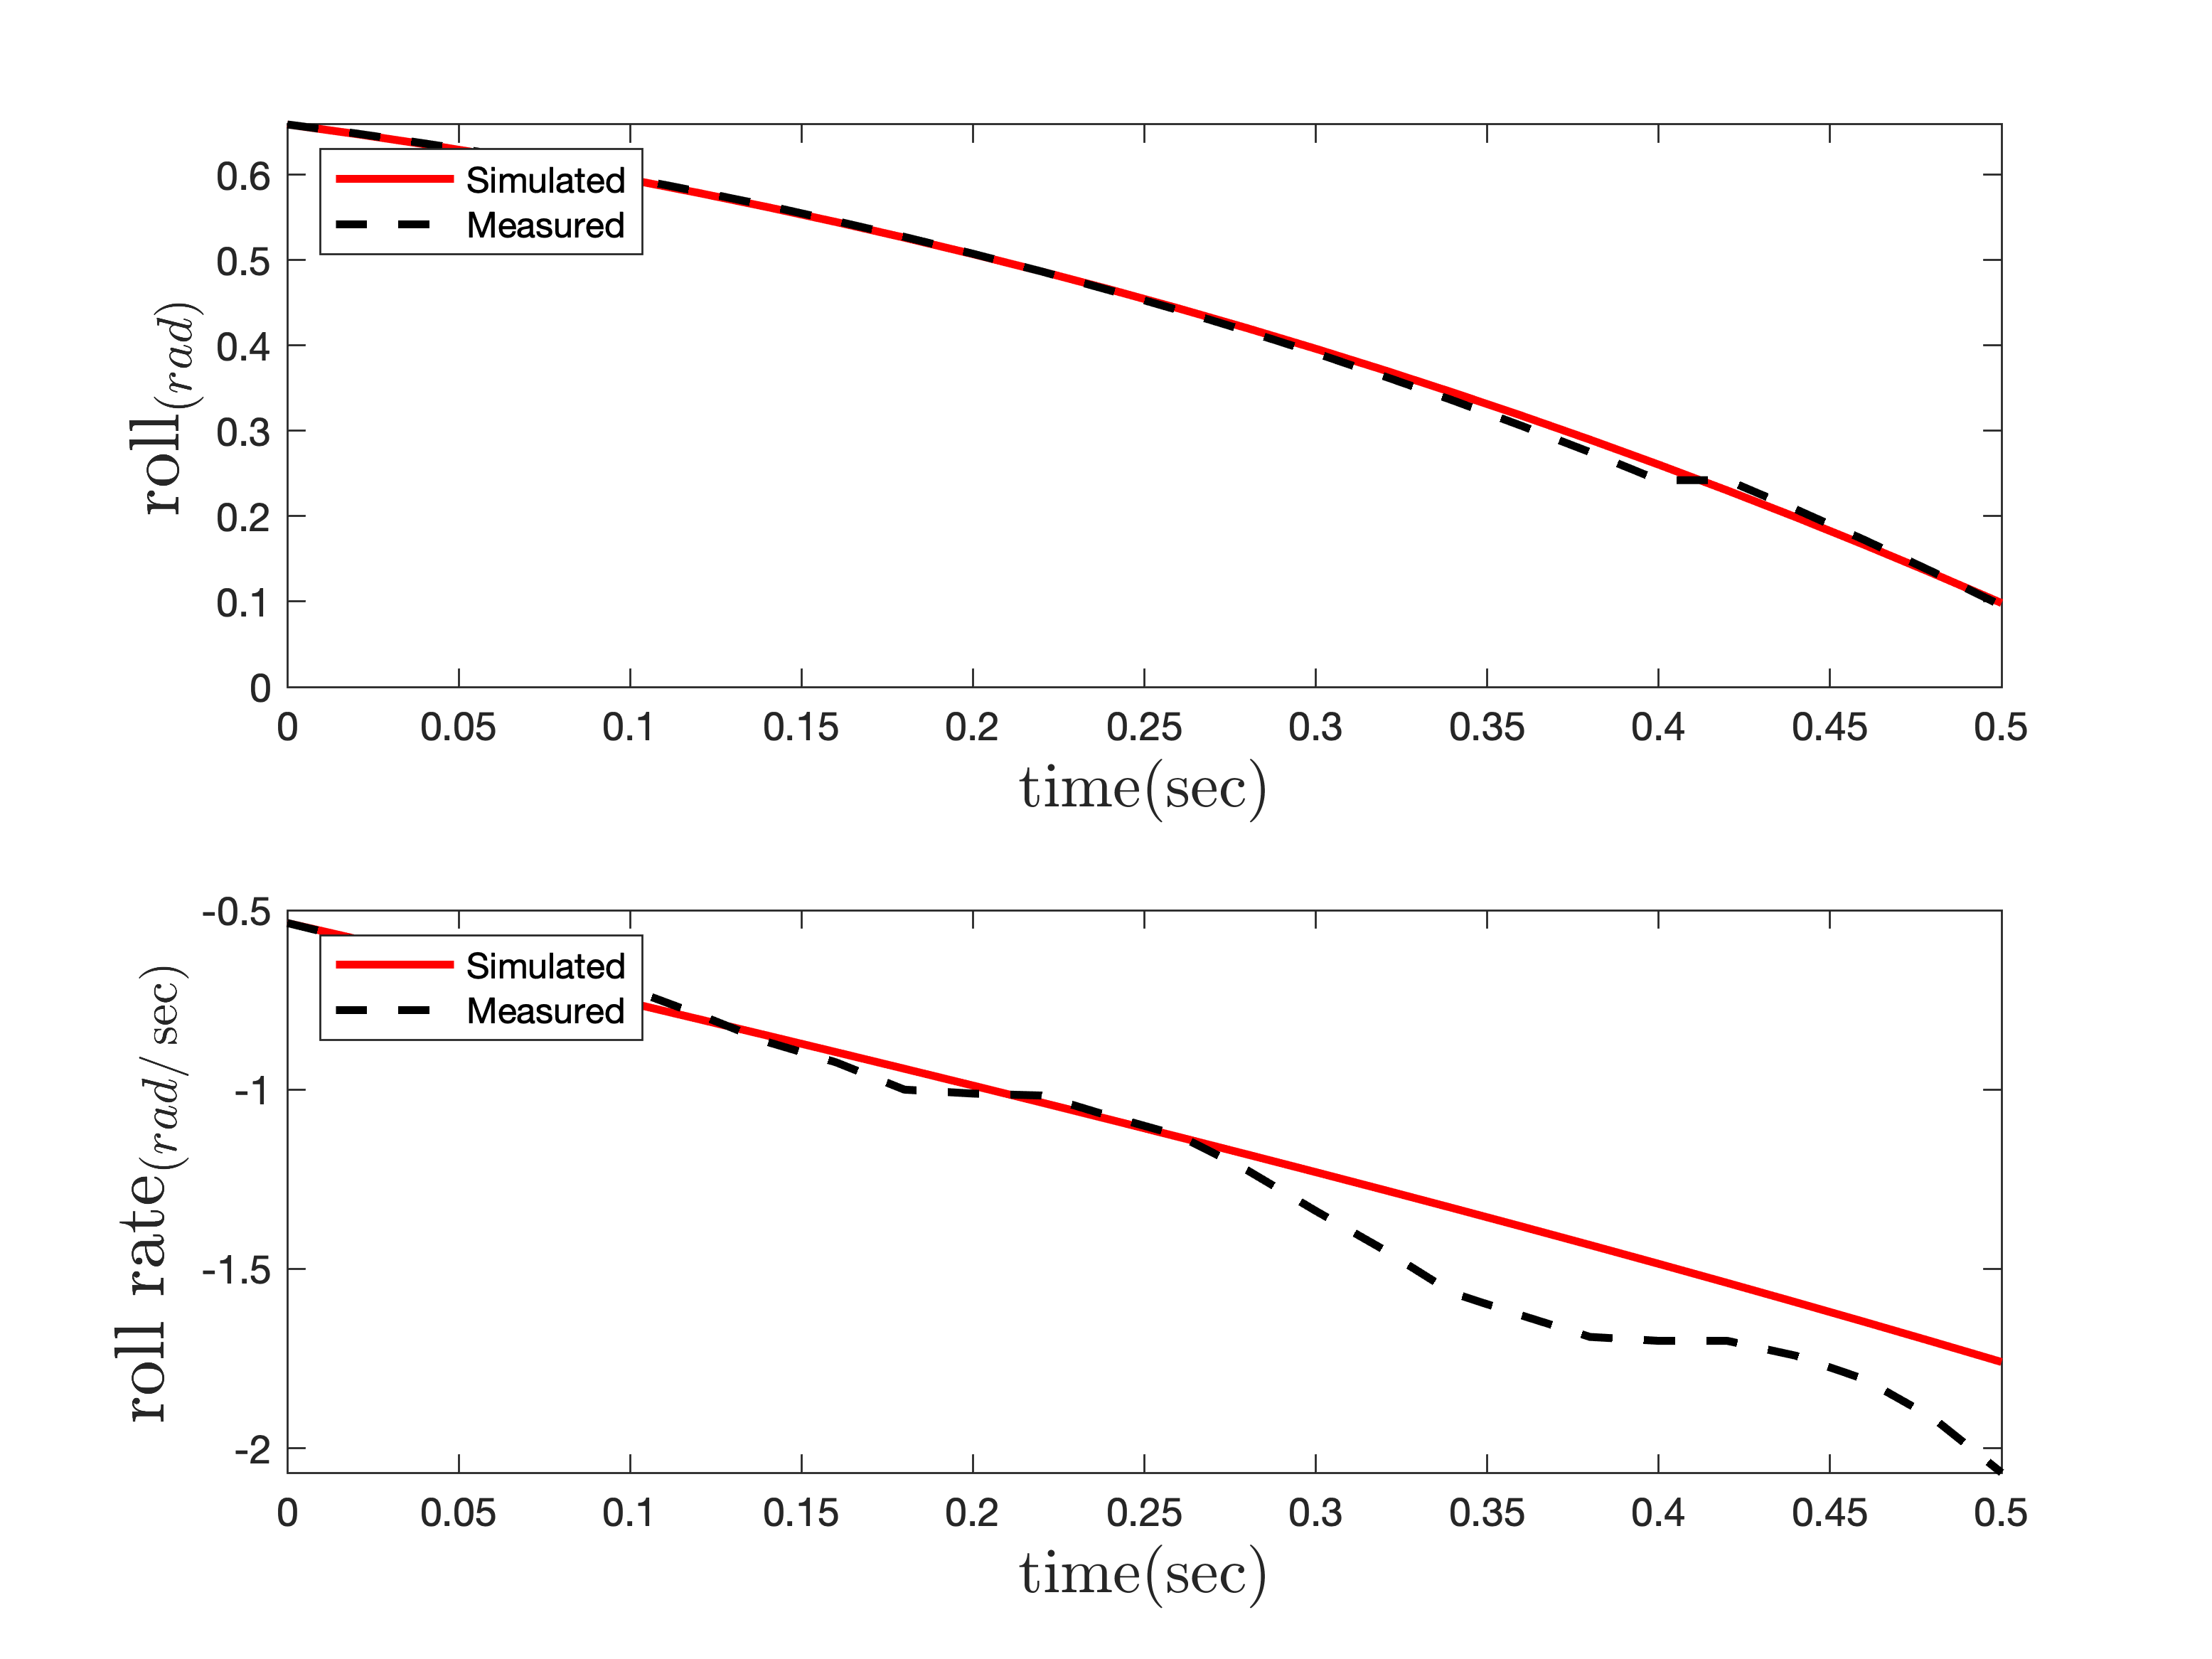
\includegraphics[width=2.32in]{../Figures/RCP/roll_parameter_estimation/RCP_roll_S4.png}
    \label{fig: roll PE}}
    \hfil
    \subfloat[Pitch]{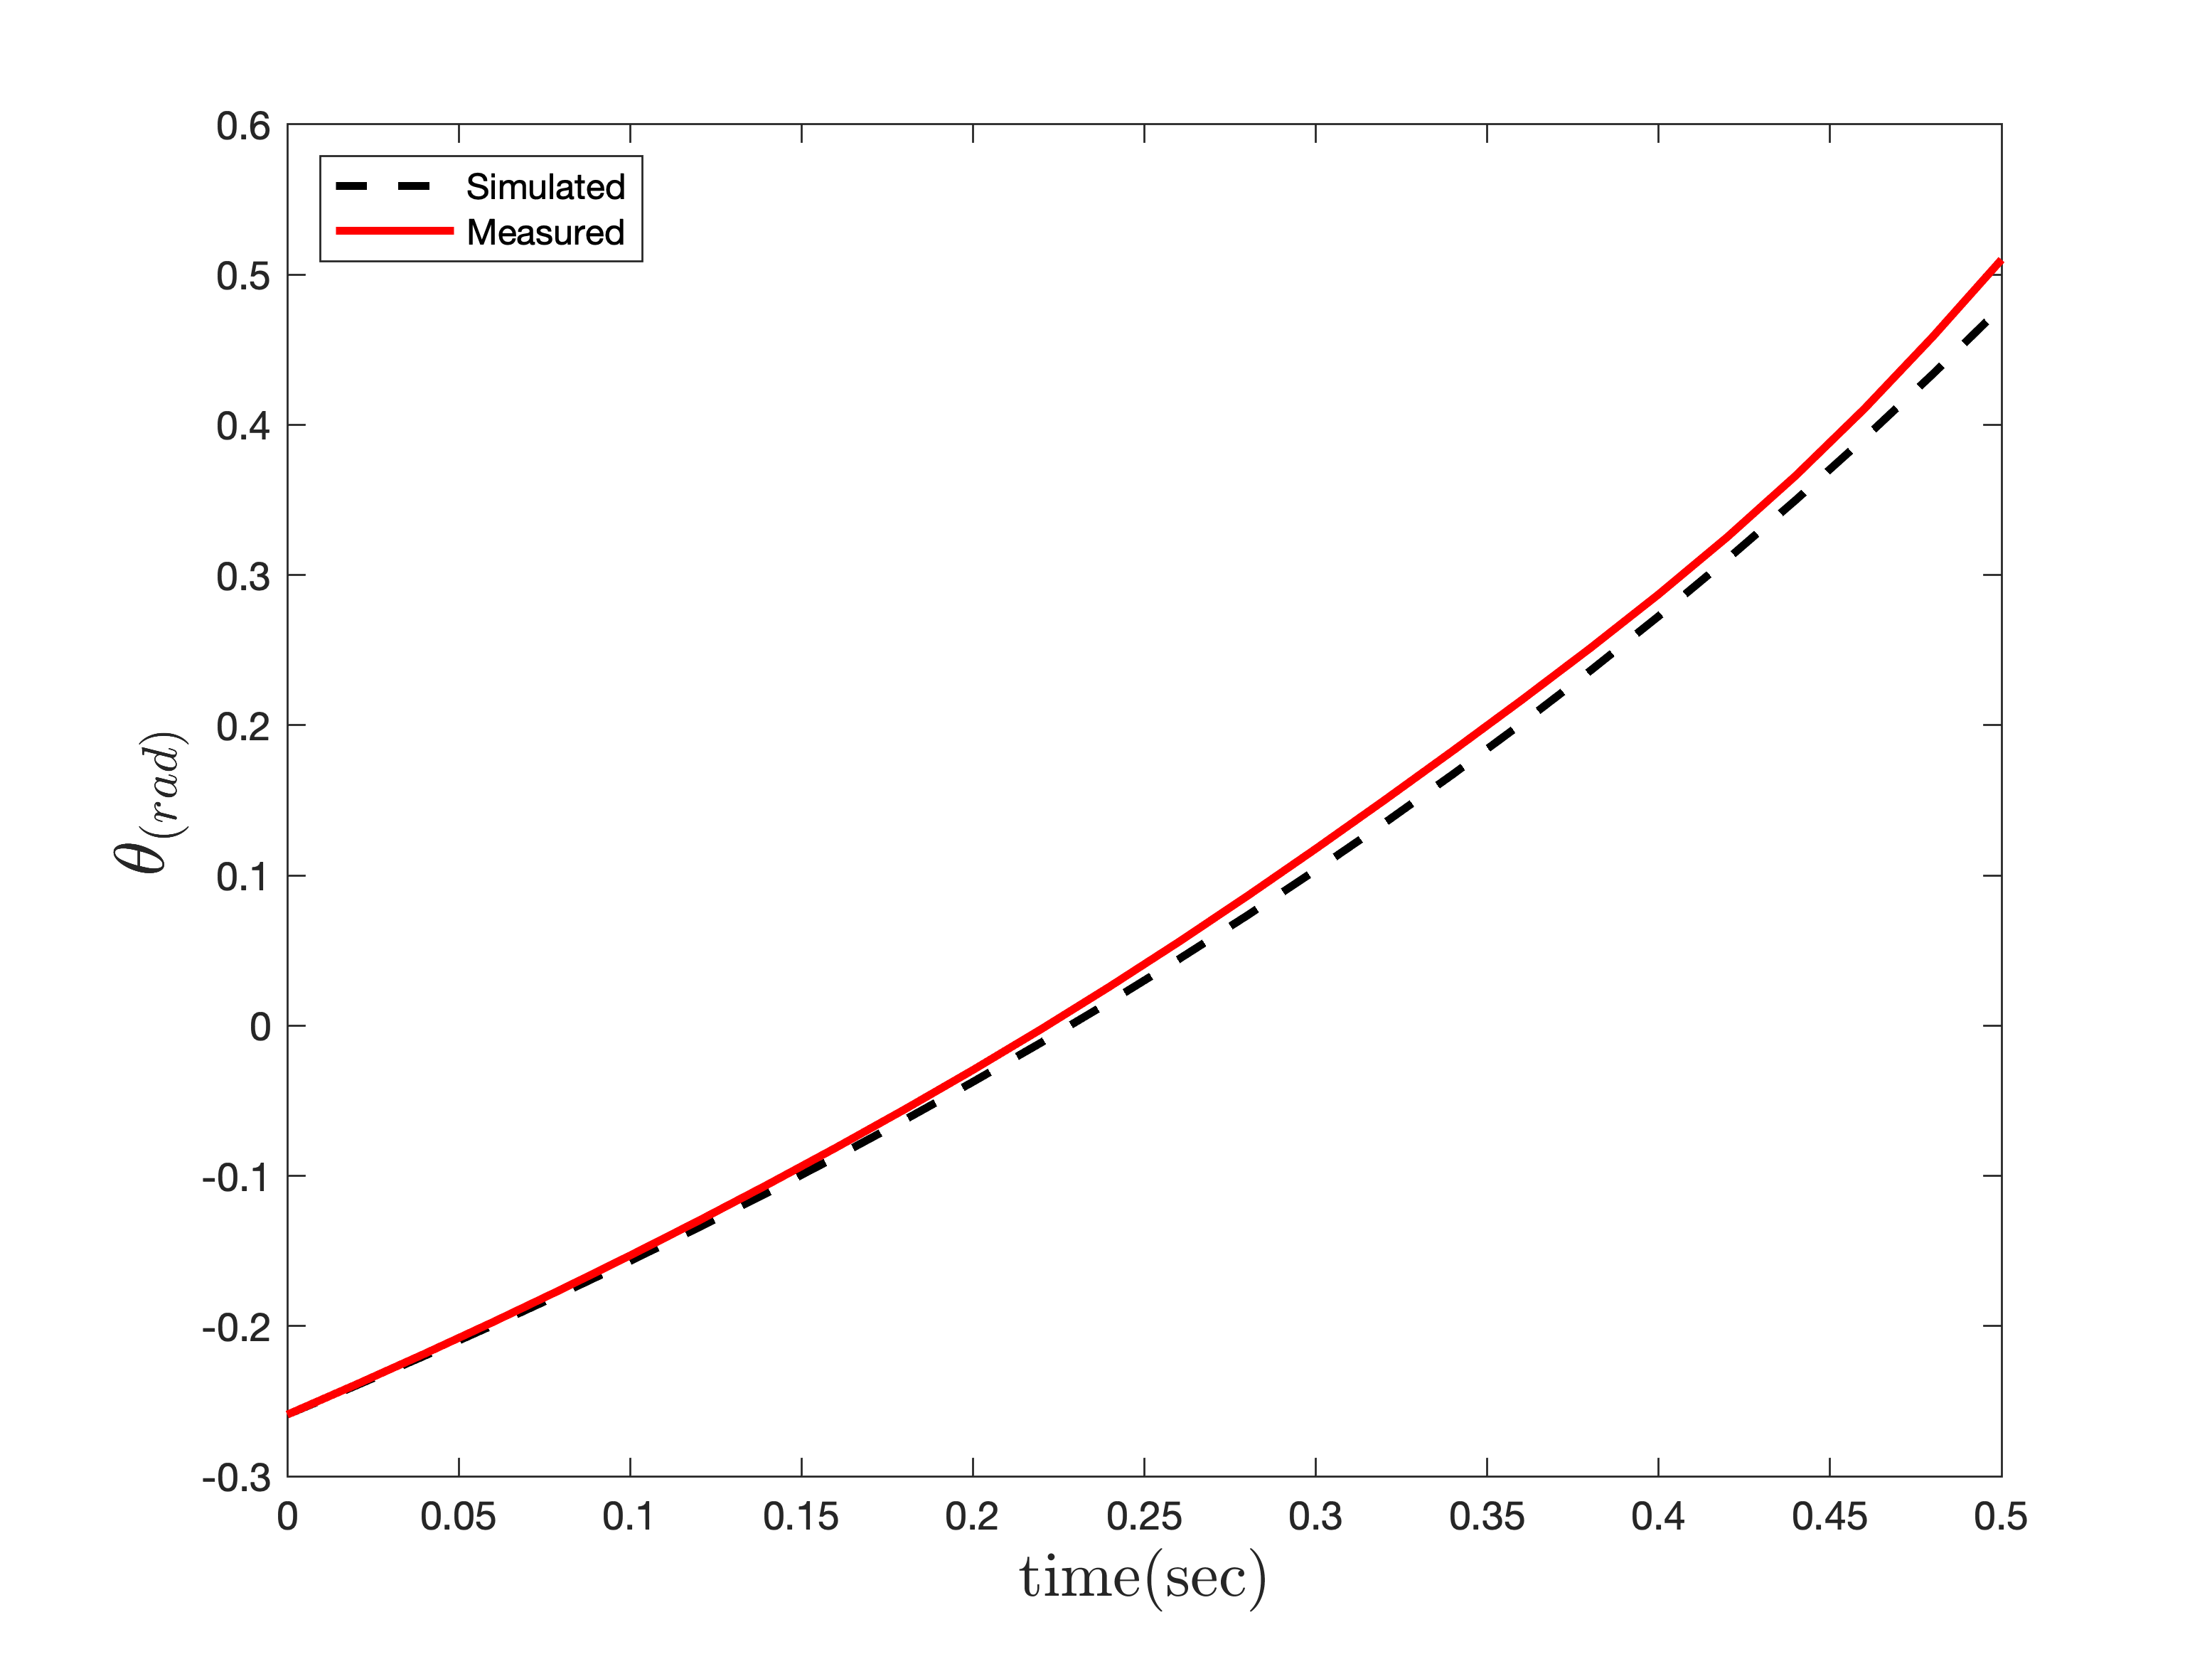
\includegraphics[width=2.32in]{../Figures/RCP/pitch_parameter_estimation/RCP_pitch_S1.png}
    \label{fig: pitch PE}}
	\hfil
    \subfloat[Yaw]{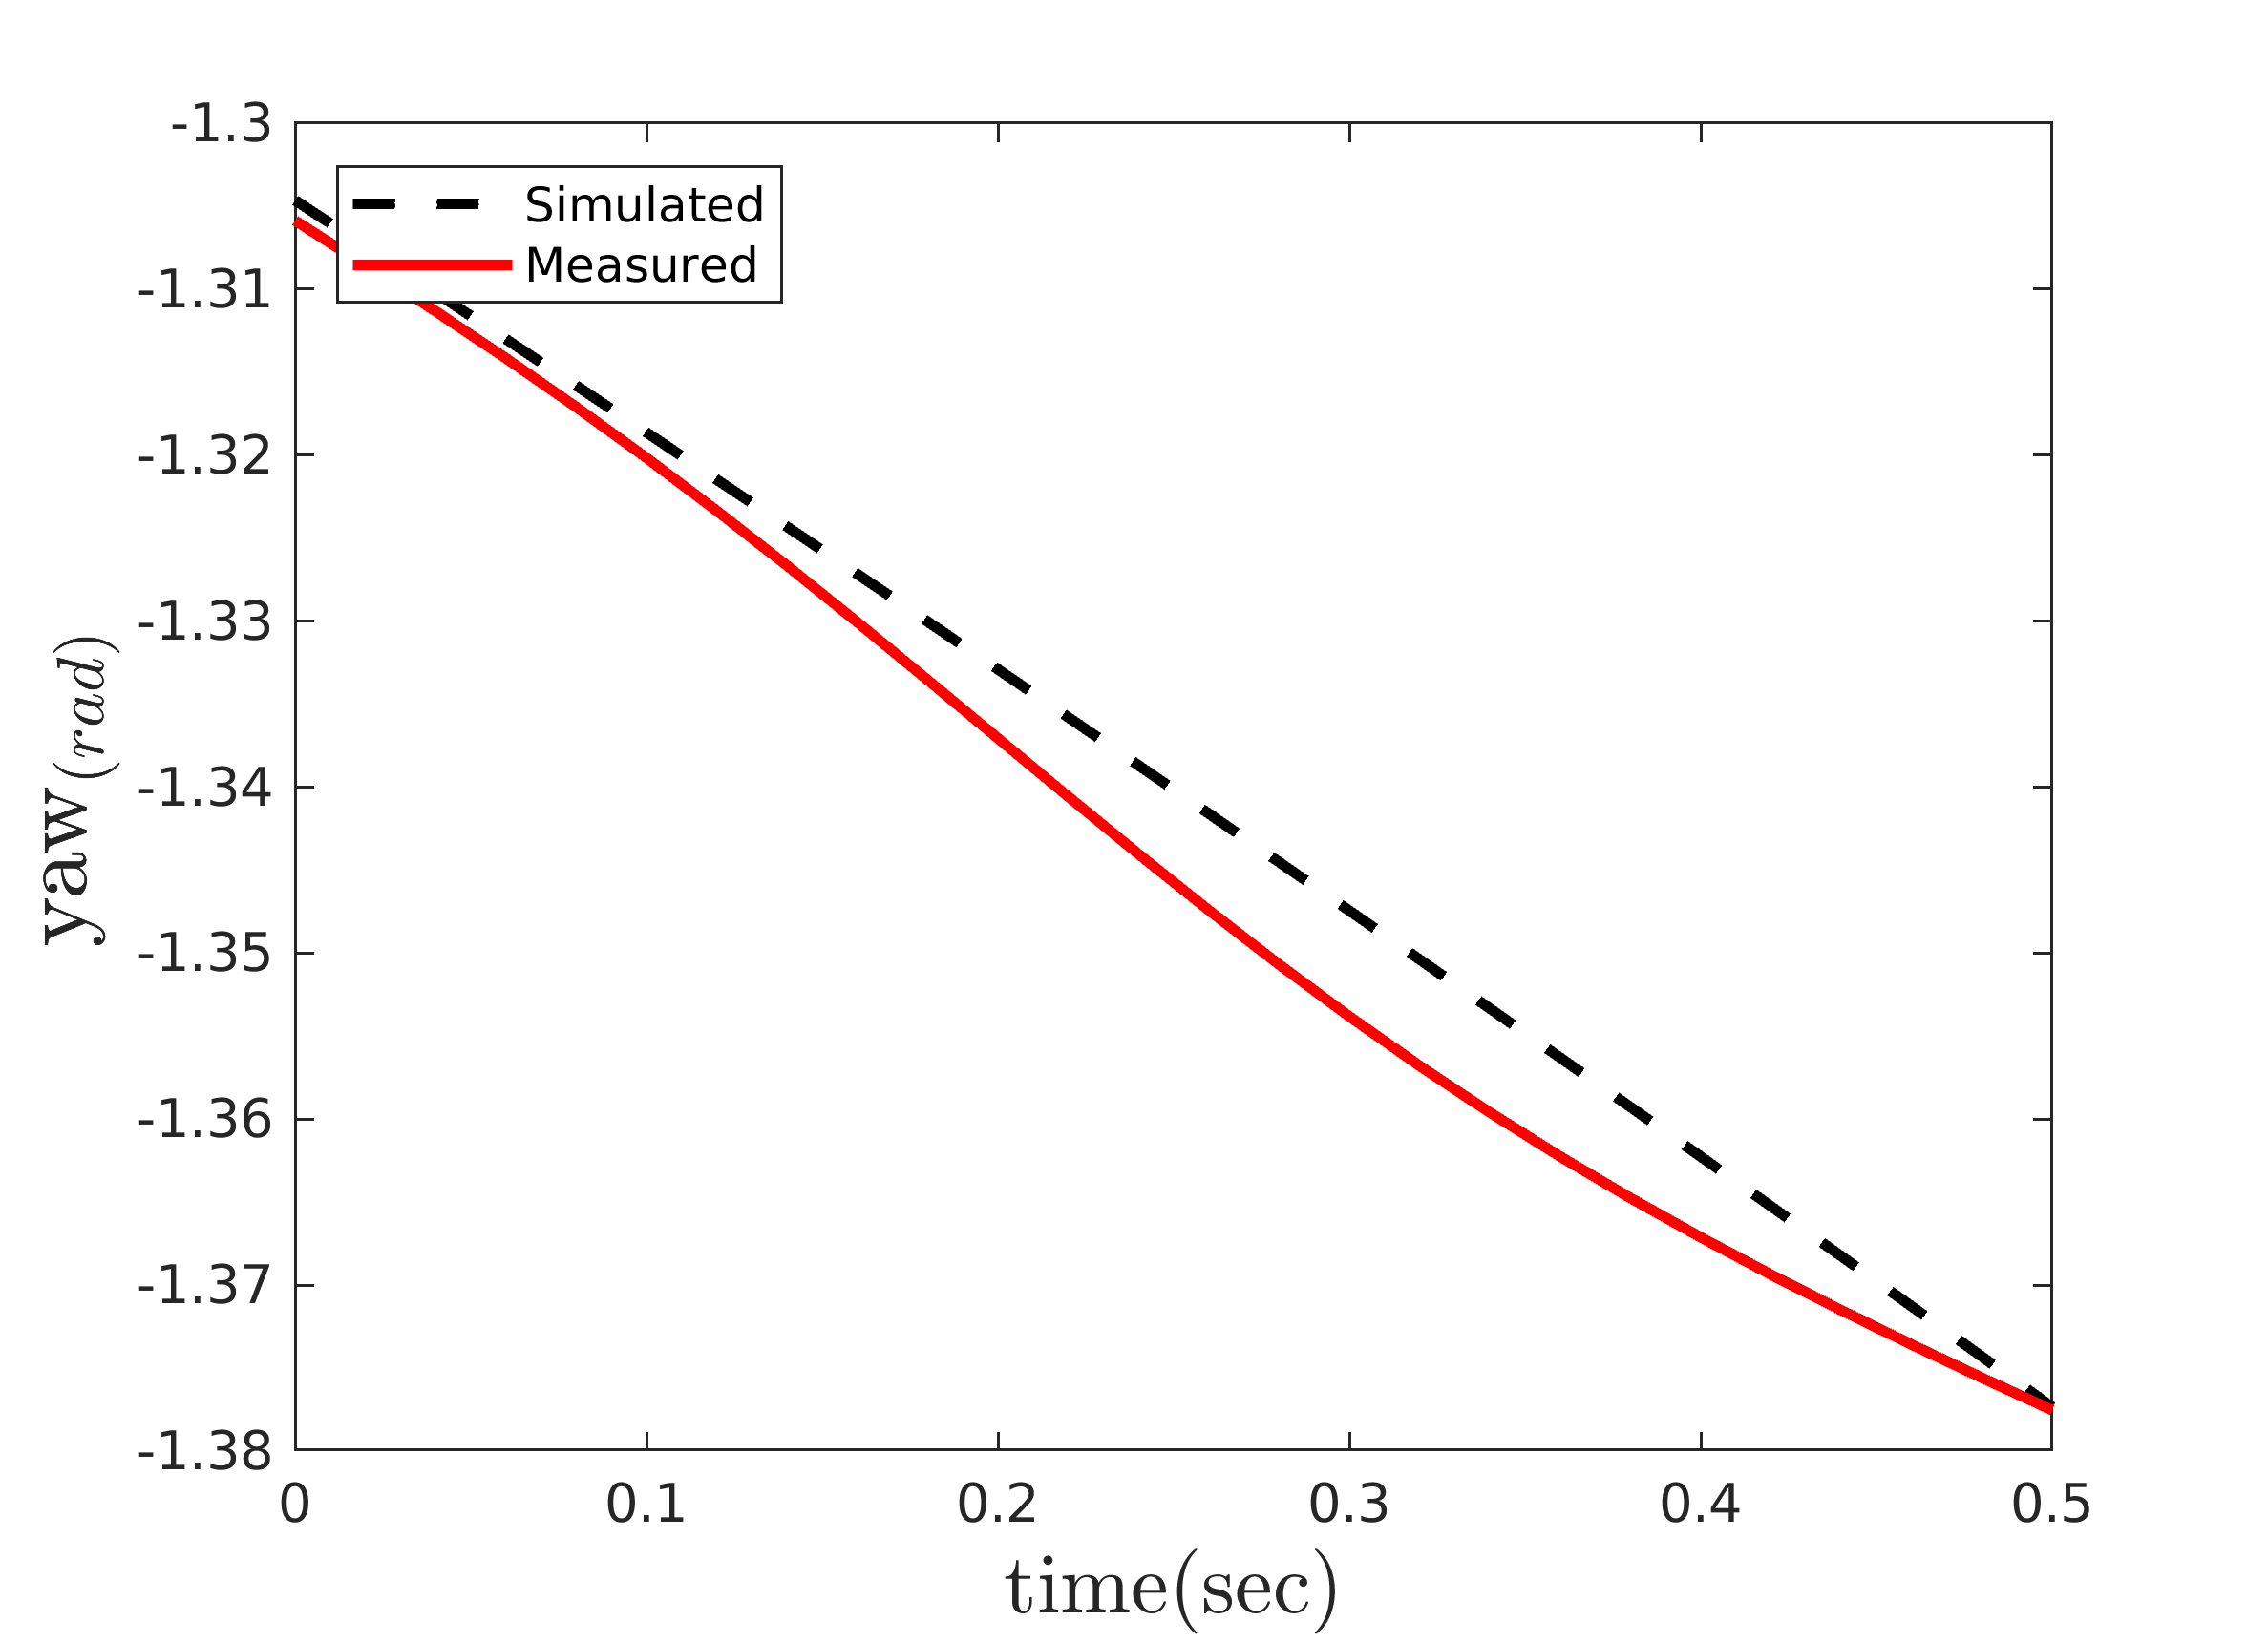
\includegraphics[width=2.32in]{../Figures/RCP/yaw_parameter_estimation/RCP_yaw_S2.png}
    \label{fig: yaw PE}}
    \caption{Simulation results for the network.} \label{fig_sim}
\end{figure*}















% \begin{figure*}[htbp]
%     \centering
%     \subfloat[Case I]{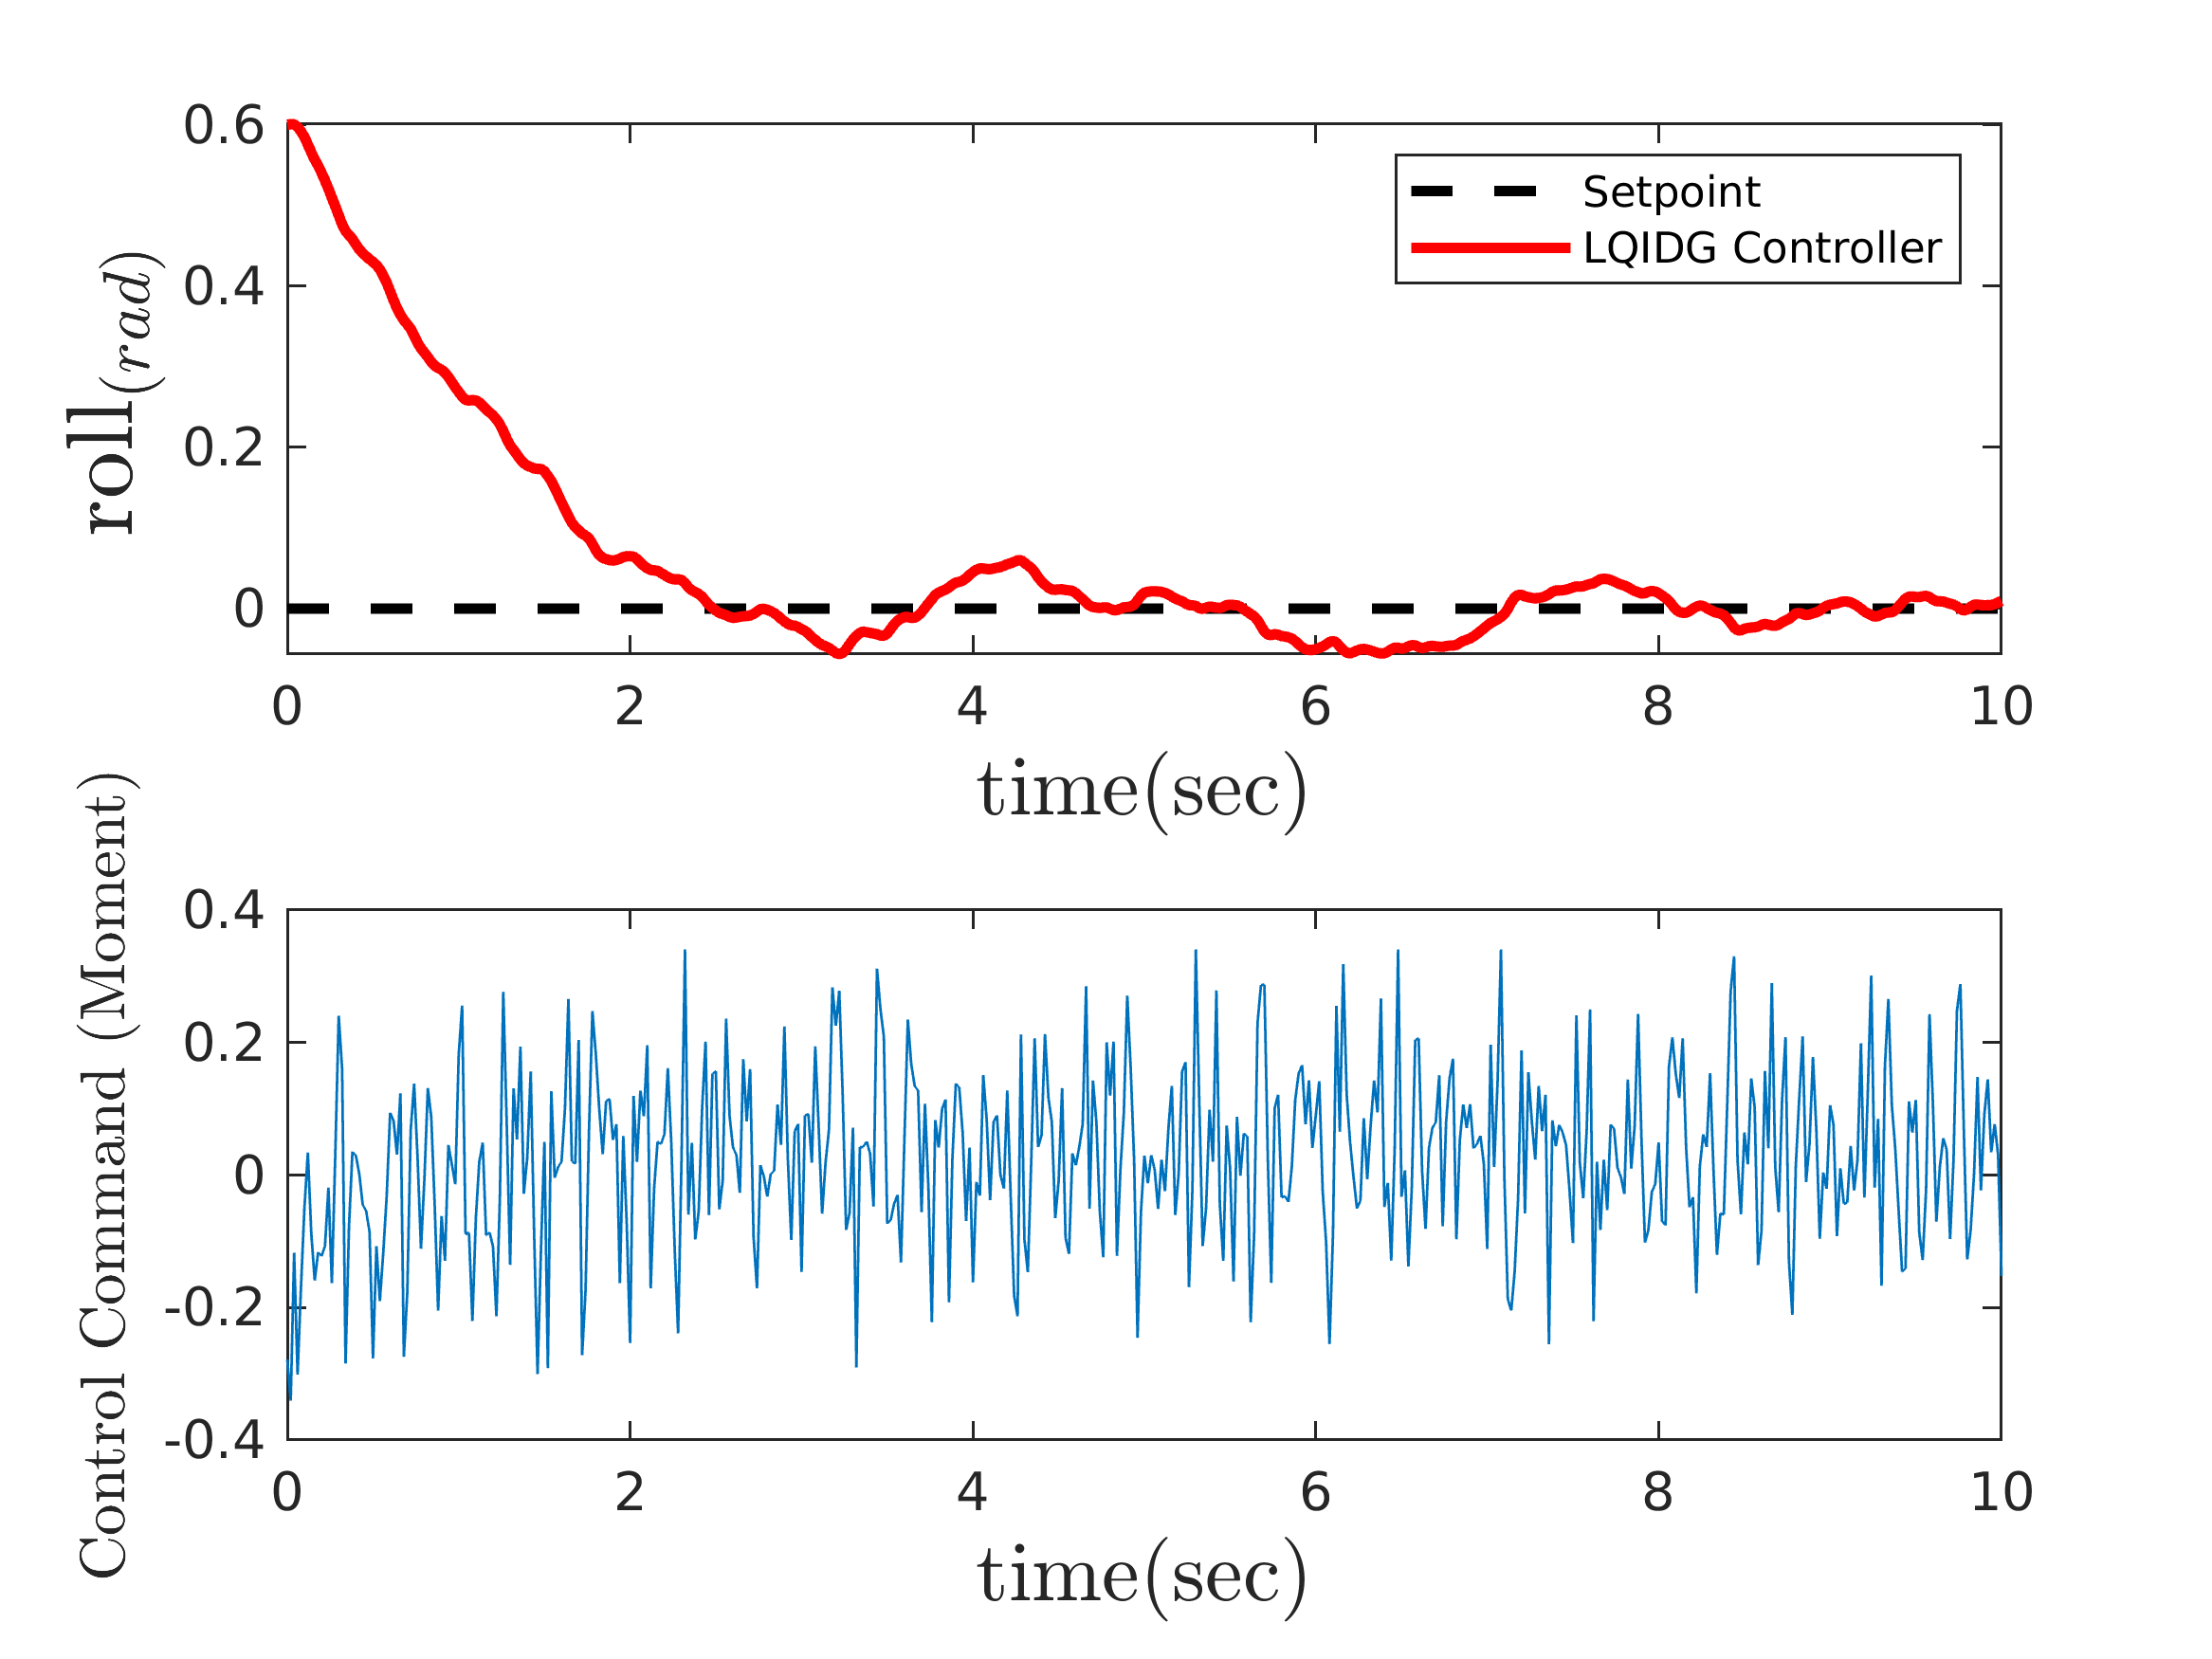
\includegraphics[width=2.5in]{../Figures/MIL/LQIDG/Roll/lqidg_roll.png}
%     \label{fig_first_case}}
%     \hfil
%     \subfloat[Case II]{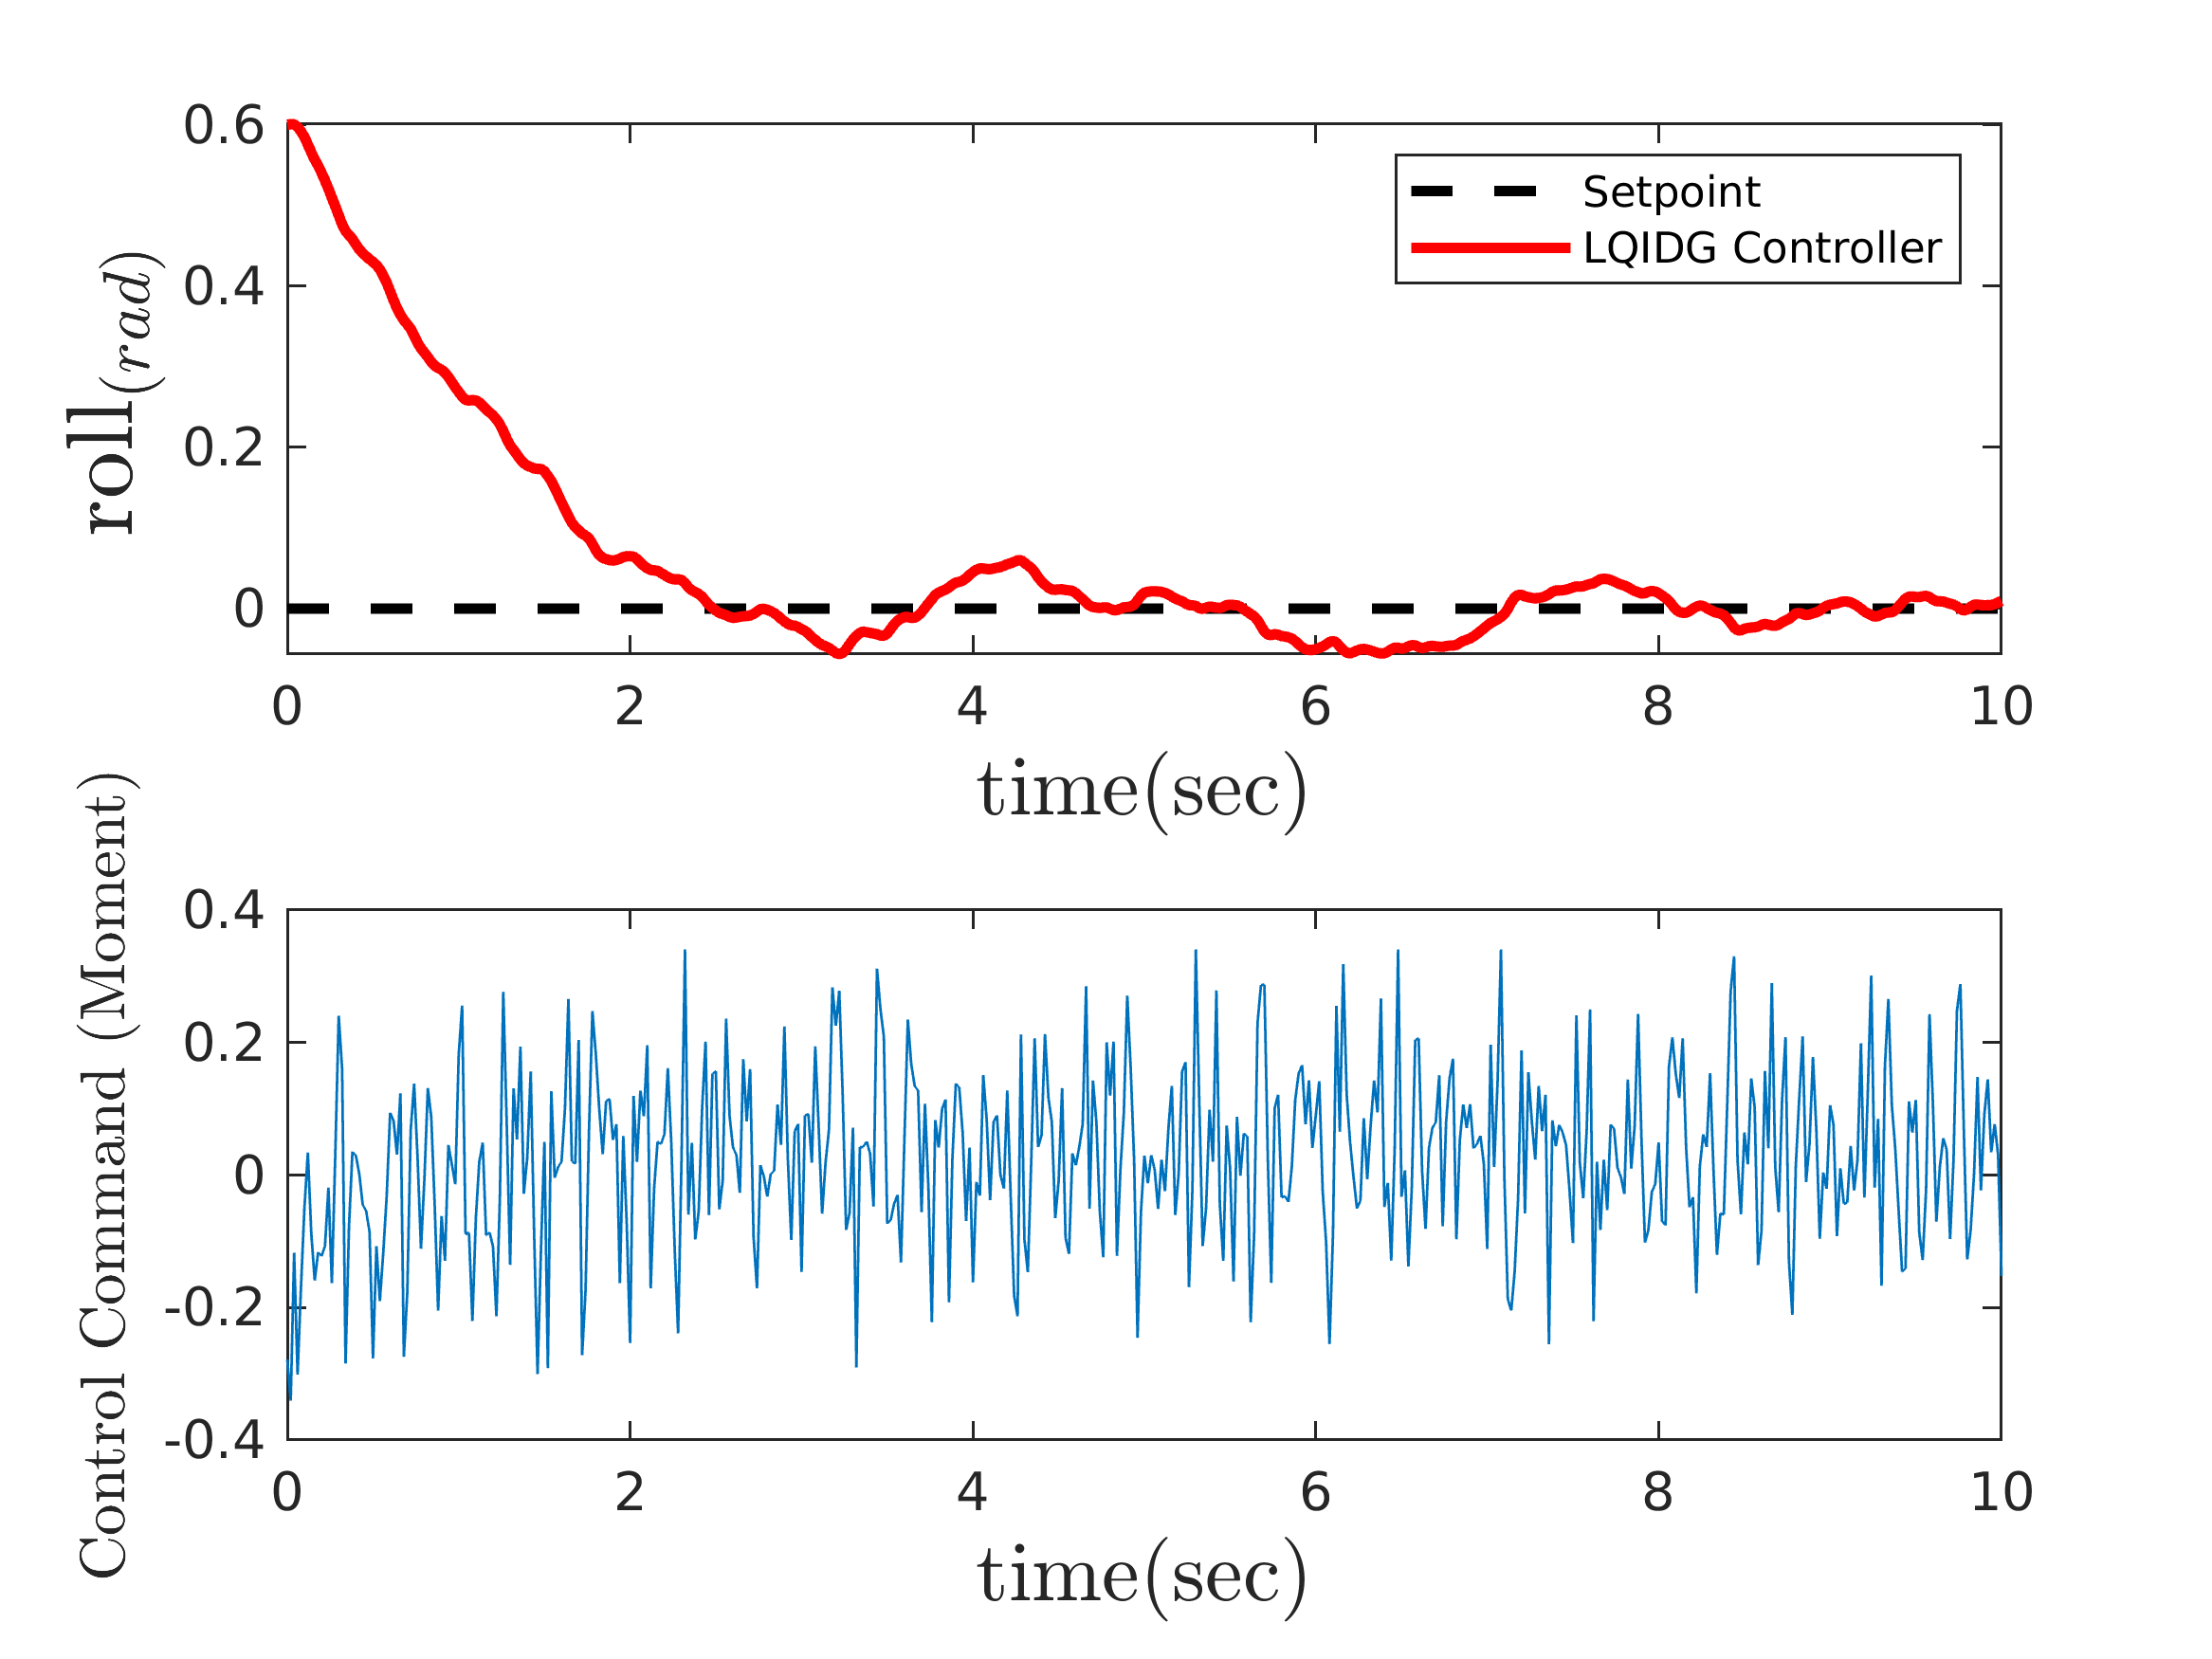
\includegraphics[width=2.5in]{../Figures/MIL/LQIDG/Roll/lqidg_roll.png}
%     \label{fig_second_case}}
%     \caption{Simulation results for the network.} \label{fig_sim}
% \end{figure*}
% \begin{figure}[htbp]
% 	\centerline{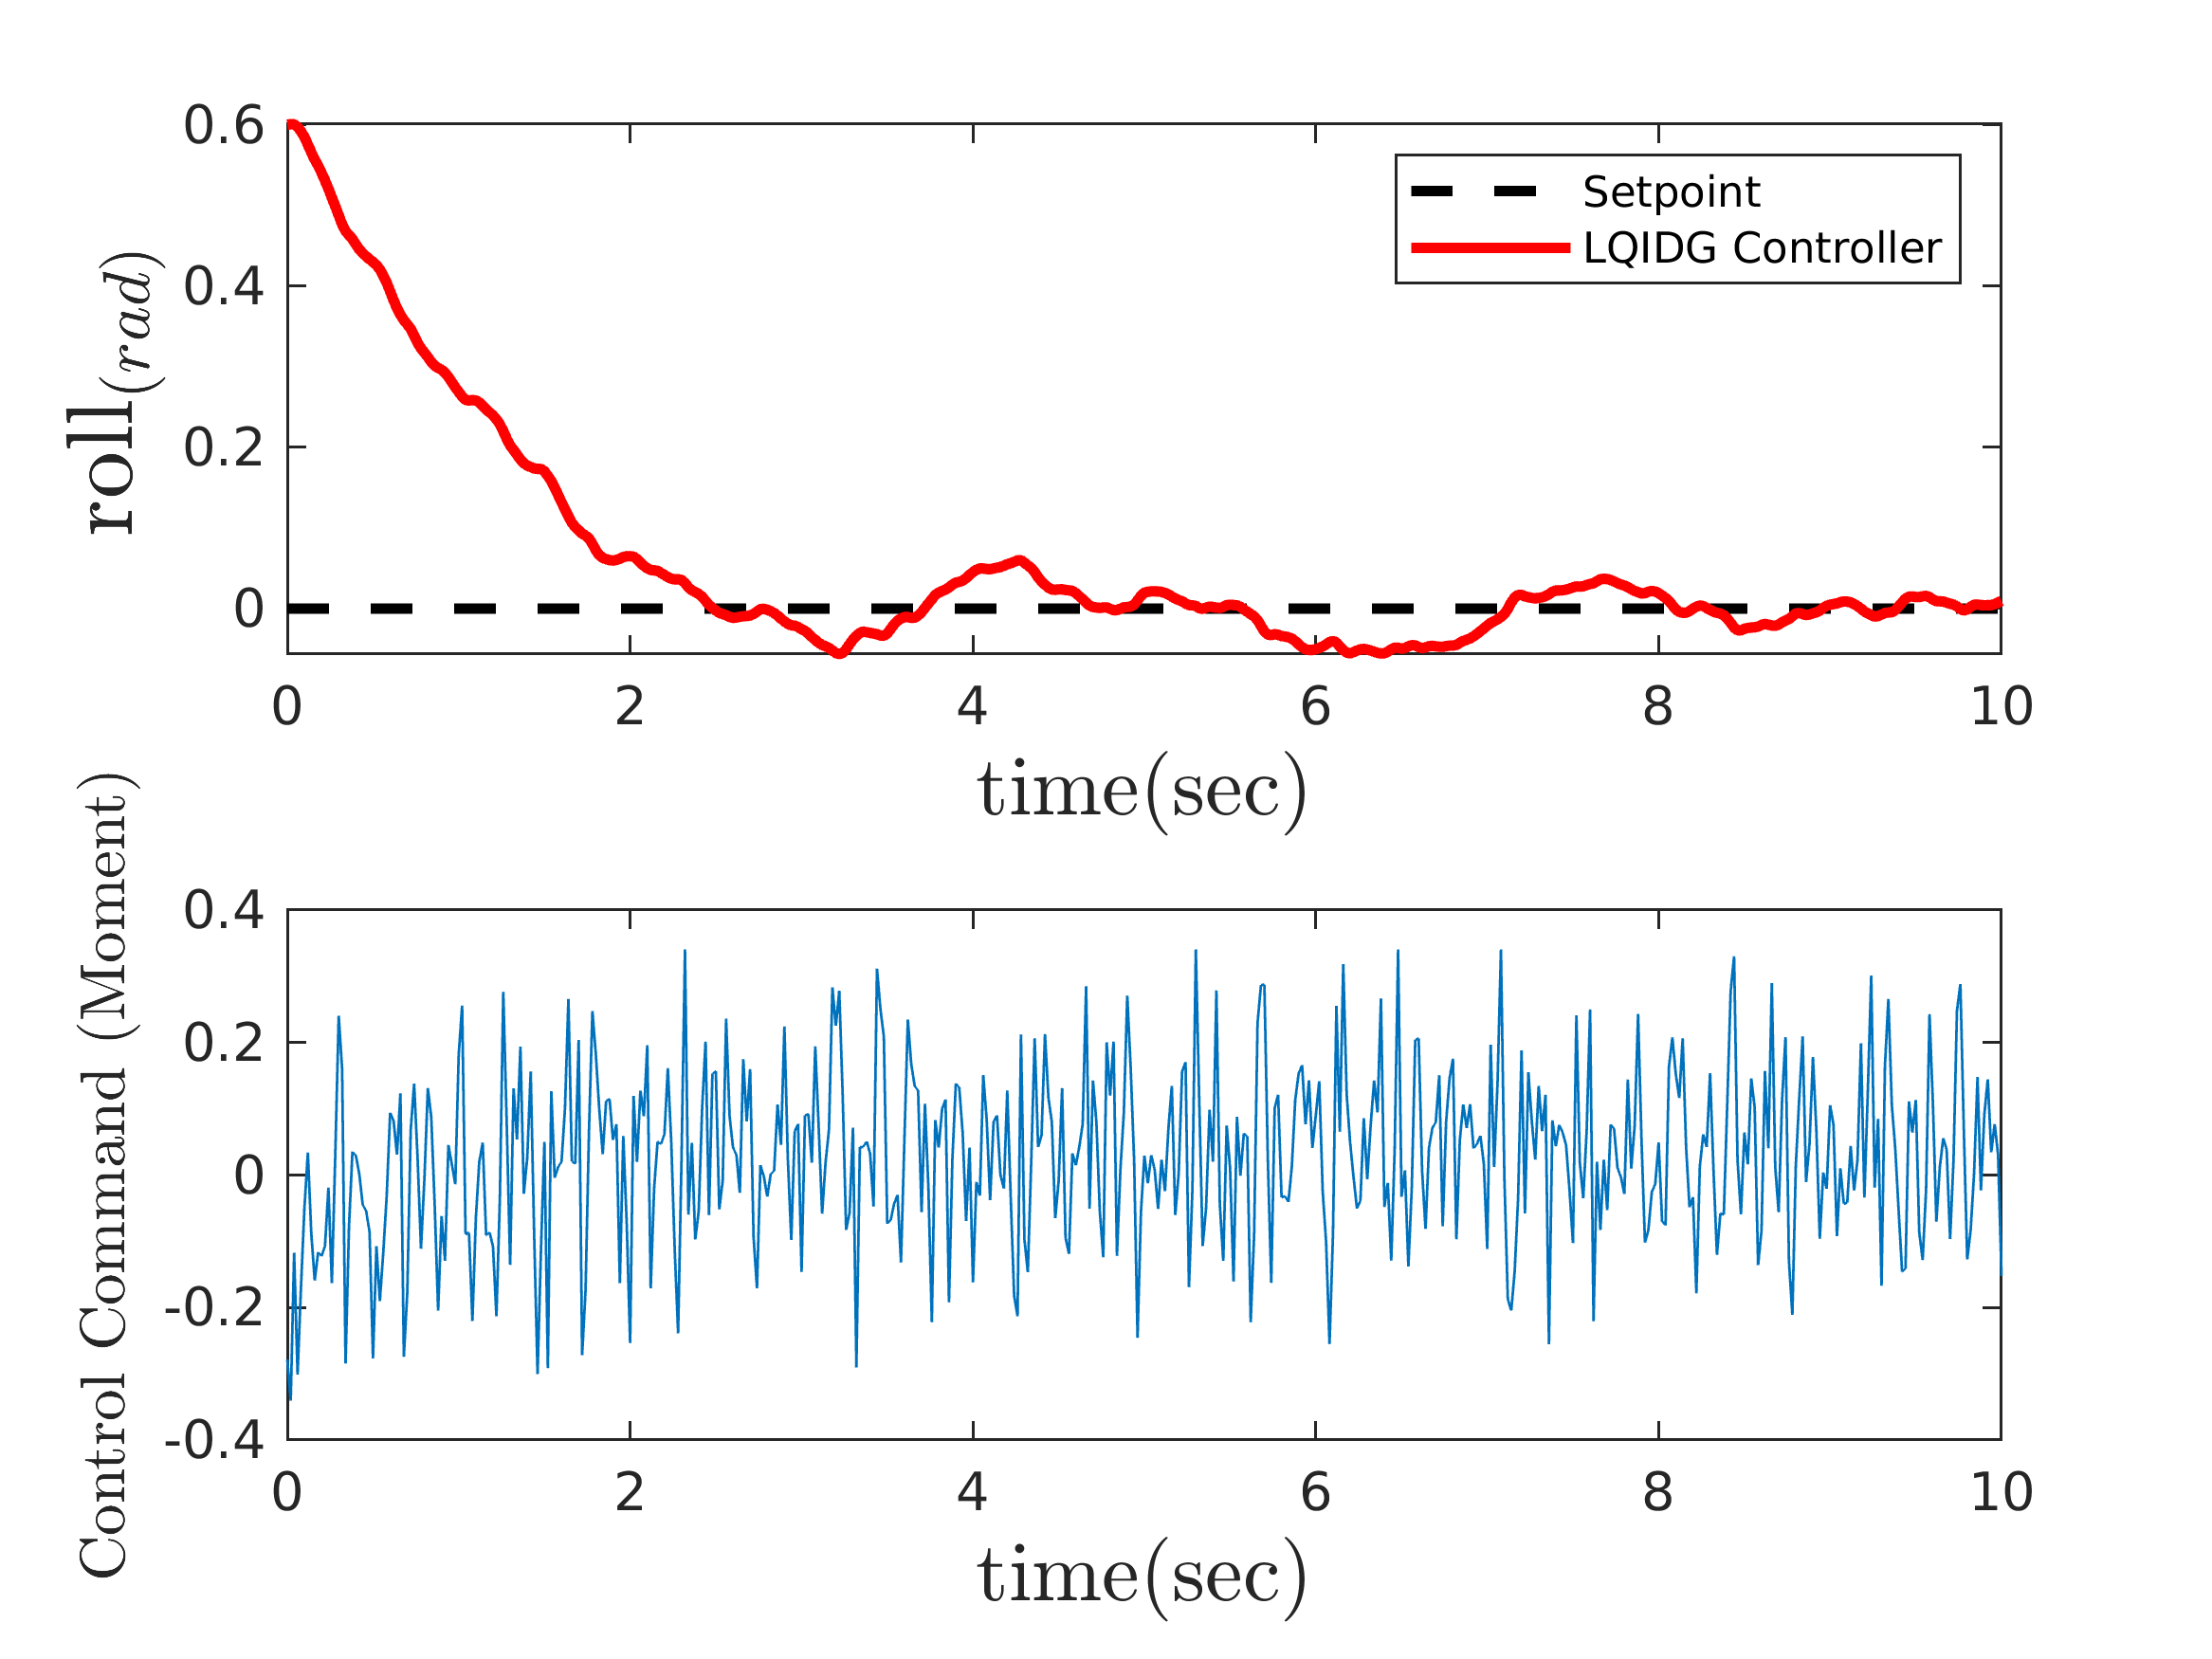
\includegraphics[width=2.5in]{../Figures/MIL/LQIDG/Roll/lqidg_roll.png}}
% 	\caption{Example of a figure caption.}
% 	\label{fig}
% \end{figure}



Before you begin to format your paper, first write and save the content as a 
separate text file. Complete all content and organizational editing before 
formatting. Please note sections \eqref{AA}--\eqref{SCM} below for more information on 
proofreading, spelling and grammar.
Keep your text and graphic files separate until after the text has been 
formatted and styled. Do not number text heads---{\LaTeX} will do that 
for you.
\subsection{Abbreviations and Acronyms}\label{AA}
Define abbreviations and acronyms the first time they are used in the text, 
even after they have been defined in the abstract. Abbreviations such as 
IEEE, SI, MKS, CGS, ac, dc, and rms do not have to be defined. Do not use 
abbreviations in the title or heads unless they are unavoidable.

\subsection{Units}
\begin{itemize}
\item Use either SI (MKS) or CGS as primary units. (SI units are encouraged.) English units may be used as secondary units (in parentheses). An exception would be the use of English units as identifiers in trade, such as ``3.5-inch disk drive''.
\item Avoid combining SI and CGS units, such as current in amperes and magnetic field in oersteds. This often leads to confusion because equations do not balance dimensionally. If you must use mixed units, clearly state the units for each quantity that you use in an equation.
\item Do not mix complete spellings and abbreviations of units: ``Wb/m\textsuperscript{2}'' or ``webers per square meter'', not ``webers/m\textsuperscript{2}''. Spell out units when they appear in text: ``. . . a few henries'', not ``. . . a few H''.
\item Use a zero before decimal points: ``0.25'', not ``.25''. Use ``cm\textsuperscript{3}'', not ``cc''.)
\end{itemize}

\subsection{Equations}
Number equations consecutively. To make your 
equations more compact, you may use the solidus (~/~), the exp function, or 
appropriate exponents. Italicize Roman symbols for quantities and variables, 
but not Greek symbols. Use a long dash rather than a hyphen for a minus 
sign. Punctuate equations with commas or periods when they are part of a 
sentence, as in:
\begin{equation}
a+b=\gamma\label{eq}
\end{equation}

Be sure that the 
symbols in your equation have been defined before or immediately following 
the equation. Use ``\eqref{eq}'', not ``Eq.~\eqref{eq}'' or ``equation \eqref{eq}'', except at 
the beginning of a sentence: ``Equation \eqref{eq} is . . .''

\subsection{\LaTeX-Specific Advice}

Please use ``soft'' (e.g., \verb|\eqref{Eq}|) cross references instead
of ``hard'' references (e.g., \verb|(1)|). That will make it possible
to combine sections, add equations, or change the order of figures or
citations without having to go through the file line by line.

Please don't use the \verb|{eqnarray}| equation environment. Use
\verb|{align}| or \verb|{IEEEeqnarray}| instead. The \verb|{eqnarray}|
environment leaves unsightly spaces around relation symbols.

Please note that the \verb|{subequations}| environment in {\LaTeX}
will increment the main equation counter even when there are no
equation numbers displayed. If you forget that, you might write an
article in which the equation numbers skip from (17) to (20), causing
the copy editors to wonder if you've discovered a new method of
counting.

{\BibTeX} does not work by magic. It doesn't get the bibliographic
data from thin air but from .bib files. If you use {\BibTeX} to produce a
bibliography you must send the .bib files. 

{\LaTeX} can't read your mind. If you assign the same label to a
subsubsection and a table, you might find that Table I has been cross
eqreferenced as Table IV-B3. 

{\LaTeX} does not have precognitive abilities. If you put a
\verb|\label| command before the command that updates the counter it's
supposed to be using, the label will pick up the last counter to be
cross referenced instead. In particular, a \verb|\label| command
should not go before the caption of a figure or a table.

Do not use \verb|\nonumber| inside the \verb|{array}| environment. It
will not stop equation numbers inside \verb|{array}| (there won't be
any anyway) and it might stop a wanted equation number in the
surrounding equation.

\subsection{Some Common Mistakes}\label{SCM}
\begin{itemize}
\item The word ``data'' is plural, not singular.
\item The subscript for the permeability of vacuum $\mu_{0}$, and other common scientific constants, is zero with subscript formatting, not a lowercase letter ``o''.
\item In American English, commas, semicolons, periods, question and exclamation marks are located within quotation marks only when a complete thought or name is cited, such as a title or full quotation. When quotation marks are used, instead of a bold or italic typeface, to highlight a word or phrase, punctuation should appear outside of the quotation marks. A parenthetical phrase or statement at the end of a sentence is punctuated outside of the closing parenthesis (like this). (A parenthetical sentence is punctuated within the parentheses.)
\item A graph within a graph is an ``inset'', not an ``insert''. The word alternatively is preferred to the word ``alternately'' (unless you really mean something that alternates).
\item Do not use the word ``essentially'' to mean ``approximately'' or ``effectively''.
\item In your paper title, if the words ``that uses'' can accurately replace the word ``using'', capitalize the ``u''; if not, keep using lower-cased.
\item Be aware of the different meanings of the homophones ``affect'' and ``effect'', ``complement'' and ``compliment'', ``discreet'' and ``discrete'', ``principal'' and ``principle''.
\item Do not confuse ``imply'' and ``infer''.
\item The prefix ``non'' is not a word; it should be joined to the word it modifies, usually without a hyphen.
\item There is no period after the ``et'' in the Latin abbreviation ``et al.''.
\item The abbreviation ``i.e.'' means ``that is'', and the abbreviation ``e.g.'' means ``for example''.
\end{itemize}
An excellent style manual for science writers is \cite{b7}.

\subsection{Authors and Affiliations}
\textbf{The class file is designed for, but not limited to, six authors.} A 
minimum of one author is required for all conference articles. Author names 
should be listed starting from left to right and then moving down to the 
next line. This is the author sequence that will be used in future citations 
and by indexing services. Names should not be listed in columns nor group by 
affiliation. Please keep your affiliations as succinct as possible (for 
example, do not differentiate among departments of the same organization).

\subsection{Identify the Headings}
Headings, or heads, are organizational devices that guide the reader through 
your paper. There are two types: component heads and text heads.

Component heads identify the different components of your paper and are not 
topically subordinate to each other. Examples include Acknowledgments and 
References and, for these, the correct style to use is ``Heading 5''. Use 
``figure caption'' for your Figure captions, and ``table head'' for your 
table title. Run-in heads, such as ``Abstract'', will require you to apply a 
style (in this case, italic) in addition to the style provided by the drop 
down menu to differentiate the head from the text.

Text heads organize the topics on a relational, hierarchical basis. For 
example, the paper title is the primary text head because all subsequent 
material relates and elaborates on this one topic. If there are two or more 
sub-topics, the next level head (uppercase Roman numerals) should be used 
and, conversely, if there are not at least two sub-topics, then no subheads 
should be introduced.

\subsection{Figures and Tables}
\paragraph{Positioning Figures and Tables} Place figures and tables at the top and 
bottom of columns. Avoid placing them in the middle of columns. Large 
figures and tables may span across both columns. Figure captions should be 
below the figures; table heads should appear above the tables. Insert 
figures and tables after they are cited in the text. Use the abbreviation 
``Fig.~\eqref{fig}'', even at the beginning of a sentence.

\begin{table}[htbp]
\caption{Table Type Styles}
\begin{center}
\begin{tabular}{|c|c|c|c|}
\hline
\textbf{Table}&\multicolumn{3}{|c|}{\textbf{Table Column Head}} \\
\cline{2-4} 
\textbf{Head} & \textbf{\textit{Table column subhead}}& \textbf{\textit{Subhead}}& \textbf{\textit{Subhead}} \\
\hline
copy& More table copy$^{\mathrm{a}}$& &  \\
\hline
\multicolumn{4}{l}{$^{\mathrm{a}}$Sample of a Table footnote.}
\end{tabular}
\label{tab1}
\end{center}
\end{table}

\begin{figure}[htbp]
\centerline{
\includegraphics{fig1.png}}
\caption{Example of a figure caption.}
\label{fig}
\end{figure}

Figure Labels: Use 8 point Times New Roman for Figure labels. Use words 
rather than symbols or abbreviations when writing Figure axis labels to 
avoid confusing the reader. As an example, write the quantity 
``Magnetization'', or ``Magnetization, M'', not just ``M''. If including 
units in the label, present them within parentheses. Do not label axes only 
with units. In the example, write ``Magnetization (A/m)'' or ``Magnetization 
\{A[m(1)]\}'', not just ``A/m''. Do not label axes with a ratio of 
quantities and units. For example, write ``Temperature (K)'', not 
``Temperature/K''.

\section*{Acknowledgment}

The peqreferred spelling of the word ``acknowledgment'' in America is without 
an ``e'' after the ``g''. Avoid the stilted expression ``one of us (R. B. 
G.) thanks $\ldots$''. Instead, try ``R. B. G. thanks$\ldots$''. Put sponsor 
acknowledgments in the unnumbered footnote on the first page.

\section*{eqreferences}

Please number citations consecutively within brackets \cite{b1}. The 
sentence punctuation follows the bracket \cite{b2}. eqrefer simply to the eqreference 
number, as in \cite{b3}---do not use ``eqref. \cite{b3}'' or ``eqreference \cite{b3}'' except at 
the beginning of a sentence: ``eqreference \cite{b3} was the first $\ldots$''

Number footnotes separately in superscripts. Place the actual footnote at 
the bottom of the column in which it was cited. Do not put footnotes in the 
abstract or eqreference list. Use letters for table footnotes.

Unless there are six authors or more give all authors' names; do not use 
``et al.''. Papers that have not been published, even if they have been 
submitted for publication, should be cited as ``unpublished'' \cite{b4}. Papers 
that have been accepted for publication should be cited as ``in press'' \cite{b5}. 
Capitalize only the first word in a paper title, except for proper nouns and 
element symbols.

For papers published in translation journals, please give the English 
citation first, followed by the original foreign-language citation \cite{b6}.

\begin{thebibliography}{00}
\bibitem{b1} G. Eason, B. Noble, and I. N. Sneddon, ``On certain integrals of Lipschitz-Hankel type involving products of Bessel functions,'' Phil. Trans. Roy. Soc. London, vol. A247, pp. 529--551, April 1955.
\bibitem{b2} J. Clerk Maxwell, A Treatise on Electricity and Magnetism, 3rd ed., vol. 2. Oxford: Clarendon, 1892, pp.68--73.
\bibitem{b3} I. S. Jacobs and C. P. Bean, ``Fine particles, thin films and exchange anisotropy,'' in Magnetism, vol. III, G. T. Rado and H. Suhl, Eds. New York: Academic, 1963, pp. 271--350.
\bibitem{b4} K. Elissa, ``Title of paper if known,'' unpublished.
\bibitem{b5} R. Nicole, ``Title of paper with only first word capitalized,'' J. Name Stand. Abbrev., in press.
\bibitem{b6} Y. Yorozu, M. Hirano, K. Oka, and Y. Tagawa, ``Electron spectroscopy studies on magneto-optical media and plastic substrate interface,'' IEEE Transl. J. Magn. Japan, vol. 2, pp. 740--741, August 1987 [Digests 9th Annual Conf. Magnetics Japan, p. 301, 1982].
\bibitem{b7} M. Young, The Technical Writer's Handbook. Mill Valley, CA: University Science, 1989.
\end{thebibliography}
\vspace{12pt}
\color{red}
IEEE conference templates contain guidance text for composing and formatting conference papers. Please ensure that all template text is removed from your conference paper prior to submission to the conference. Failure to remove the template text from your paper may result in your paper not being published.

\end{document}
